 
\chapter{Analise e especificação}

Na proposta de sistema está contido a descrição do modelo de negócio, onde serão identificados os principais
 problemas do modelo atual e será indicada a necessidade de implementação do software. Nesta proposta 
 estará também identificado os objetivos de negócio, conseguindo identificar o principal impacto deste 
 software neste modelo de negócio. Nesta proposta estará também contida a engenharia de software com toda 
 a especificação do projeto em mãos.


 \section{Modelo de negócio}

Este projeto surgiu com a necessidade da Motorline melhorar a comunicação e a experiência das 
empresas clientes e técnicos. 
Atualmente sempre que um técnico possui uma questão este deverá contactar o suporte técnico o que pode 
levar a sobrecarga deste, ou então este deverá se juntar ao grupo do Facebook de técnicos e colocar 
neste esta questão. Sempre que é necessário um manual de produto ou sempre que o utilizador pretender ver 
o catalogo este deverá se deslocar ao site da Motorline e procurar o produto no catálogo não possuindo um
acesso rápido a estes.
Visto que este processo acaba por não ser prático para o utilizador, foi então 
decidido suprir este problema com o projeto Install \& Go. Tendo estas questões em mente surgiu então 
a ideia de implementar um fórum de resolução de problemas.


 \section{Objetivos de negócio}

Este software visa minimizar o problema acima descrito. Visto que acontece que muitas das 
questões dos técnicos são comuns, então surgiu a ideia de implementar um fórum onde o técnico poderá 
pesquisar por questões semelhantes à sua, encontrando solução sem necessidade de contactar o suporte 
técnico. O técnico poderá também expor a sua questão anexando imagens, facilitando o processo de 
resolução da sua questão. Para existir partilha de conhecimento o técnico poderá também responder 
a tópicos, pois caso encontre alguma questão que já tenha resolvido poderá ajudar outro técnico. O técnico 
também poderá alterar a visibilidade do seu tópico caso deseje que apenas técnicos visualizem a sua questão.

A empresa poderá realizar as mesmas ações que o técnico, mas esta poderá também criar contas para os seus 
técnicos e realizar a gestão destas sendo importante permitir apagar e impedir acesso à conta em caso de 
necessidade.


 \section{Estado da arte}
 Para ser possível entender todo o negócio onde este projeto se encaixa foi realizado um estudo
 englobando outras soluções do mesmo ramo. Estas soluções investigadas foram indicação do supervisor
 de estágio pois este já teria realizado um estudo da situação do negócio préviamente.
 As soluções investigadas foram, FixAndGo, My VDS e Ultimate Cardin. A solução FixAndGo 
 foi indicada devido à capacidade de calcular a possibilidade de instalar em motor baseando-se em
 medidas indicadas pelo utilizador. Já a solução My VDS foi indicada devido a dispor documentação sobre
 os seus produtos como manuais e vídeos, assim como também uma forma de comunicação com a equipa de suporte.
 Por fim a solução Ultimate Cardin foi utilizada como exemplo de design a não seguir devido a ser confuso, 
 esta foi também utilizada como exemplo de organização de design do ecrã de detalhes de produto.

 \section{Domínio de aplicação do sistema}

Com o diagrama da Figura~\ref{fig:2} é possível visualizar todos os atores do \textit{software} e as suas ações, assim como os sistemas envolvidos na aplicação e as funções.
Destes é possível identificar que este \textit{software} contém três atores principais, o Utilizador que é um utilizador sem sessão iniciada, o Técnico, um utilizador com sessão iniciada, já a Empresa é uma empresa cliente da Motorline. Também é possível visualizar os diferentes sistemas integrados no projeto, como Servidor Motorline onde serão obtidas informações do catálogo de produtos, Servidor \textit{Install \& Go} onde estão todas as funções de suporte ao \textit{software}, o Servidor de Imagens onde serão guardadas todas as imagens da aplicação e por fim o Servidor de \textit{Email} que enviará \textit{email} com o código de validação de conta para os clientes assim que se registarem no \textit{software}.

\begin{figure}[htb]
  \centering
  
  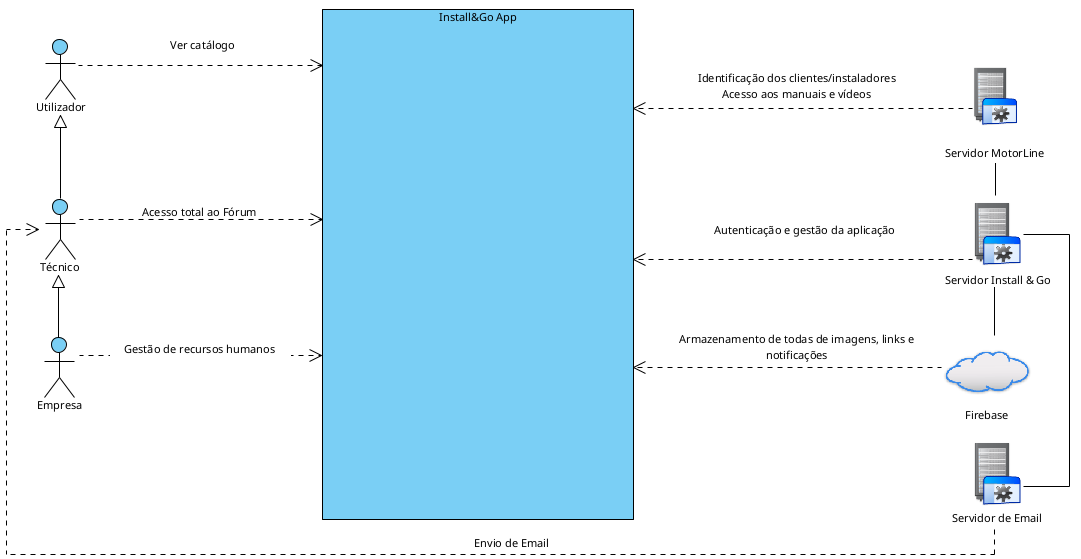
\includegraphics[width=\textwidth]{images/diagramas/diagrama_contexto.png}
  \caption{Diagrama de contexto da aplicação}
  \label{fig:2}
\end{figure}

 \newpage

 \section{Operações a realizar no sistema}
A primeira tarefa a realizar no desenvolvimento desta etapa do projeto foi o levantamento dos requisitos funcionais(Tabela~\ref{tab:1}) e não funcionais, tendo sido posteriormente validados com cliente. 

\definecolor{Mercury}{rgb}{0.905,0.901,0.901}
\begin{longtblr}
[
caption={Tabela de requisitos funcionais},
label={tab:1},
]
{
  width = \linewidth,
  colspec = {Q[75]Q[400]Q[160]Q[120]},
  row{1} = {Mercury},
  row{2} = {Mercury,c},
  row{10} = {Mercury,c},
  row{20} = {Mercury,c},
  row{26} = {Mercury,c},
  row{31} = {Mercury,c},
  row{35} = {Mercury,c},
  row{40} = {Mercury,c},
  row{45} = {Mercury,c},
  row{50} = {Mercury,c},
  cell{1}{1} = {c},
  cell{1}{3} = {c},
  cell{1}{4} = {c},
  cell{3}{1} = {c},
  cell{3}{3} = {c},
  cell{3}{4} = {c},
  cell{4}{1} = {c},
  cell{4}{3} = {c},
  cell{4}{4} = {c},
  cell{5}{1} = {c},
  cell{5}{3} = {c},
  cell{5}{4} = {c},
  cell{6}{1} = {c},
  cell{6}{3} = {c},
  cell{6}{4} = {c},
  cell{7}{1} = {c},
  cell{7}{3} = {c},
  cell{7}{4} = {c},
  cell{8}{1} = {c},
  cell{8}{3} = {c},
  cell{8}{4} = {c},
  cell{9}{1} = {c},
  cell{9}{3} = {c},
  cell{9}{4} = {c},
  cell{11}{1} = {c},
  cell{11}{3} = {c},
  cell{11}{4} = {c},
  cell{12}{1} = {c},
  cell{12}{3} = {c},
  cell{12}{4} = {c},
  cell{13}{1} = {c},
  cell{13}{3} = {c},
  cell{13}{4} = {c},
  cell{14}{1} = {c},
  cell{14}{3} = {c},
  cell{14}{4} = {c},
  cell{15}{1} = {c},
  cell{15}{3} = {c},
  cell{15}{4} = {c},
  cell{16}{1} = {c},
  cell{16}{3} = {c},
  cell{16}{4} = {c},
  cell{17}{1} = {c},
  cell{17}{3} = {c},
  cell{17}{4} = {c},
  cell{18}{1} = {c},
  cell{18}{3} = {c},
  cell{18}{4} = {c},
  cell{19}{1} = {c},
  cell{19}{3} = {c},
  cell{19}{4} = {c},
  cell{21}{1} = {c},
  cell{21}{3} = {c},
  cell{21}{4} = {c},
  cell{22}{1} = {c},
  cell{22}{3} = {c},
  cell{22}{4} = {c},
  cell{23}{1} = {c},
  cell{23}{3} = {c},
  cell{23}{4} = {c},
  cell{24}{1} = {c},
  cell{24}{3} = {c},
  cell{24}{4} = {c},
  cell{25}{1} = {c},
  cell{25}{3} = {c},
  cell{25}{4} = {c},
  cell{27}{1} = {c},
  cell{27}{3} = {c},
  cell{27}{4} = {c},
  cell{28}{1} = {c},
  cell{28}{3} = {c},
  cell{28}{4} = {c},
  cell{29}{1} = {c},
  cell{29}{3} = {c},
  cell{29}{4} = {c},
  cell{30}{1} = {c},
  cell{30}{3} = {c},
  cell{30}{4} = {c},
  cell{32}{1} = {c},
  cell{32}{3} = {c},
  cell{32}{4} = {c},
  cell{33}{1} = {c},
  cell{33}{3} = {c},
  cell{33}{4} = {c},
  cell{34}{1} = {c},
  cell{34}{3} = {c},
  cell{34}{4} = {c},
  cell{36}{1} = {c},
  cell{36}{3} = {c},
  cell{36}{4} = {c},
  cell{37}{1} = {c},
  cell{37}{3} = {c},
  cell{37}{4} = {c},
  cell{38}{1} = {c},
  cell{38}{3} = {c},
  cell{38}{4} = {c},
  cell{39}{1} = {c},
  cell{39}{3} = {c},
  cell{39}{4} = {c},
  cell{41}{1} = {c},
  cell{41}{3} = {c},
  cell{41}{4} = {c},
  cell{42}{1} = {c},
  cell{42}{3} = {c},
  cell{42}{4} = {c},
  cell{43}{1} = {c},
  cell{43}{3} = {c},
  cell{43}{4} = {c},
  cell{44}{1} = {c},
  cell{44}{3} = {c},
  cell{44}{4} = {c},
  cell{46}{1} = {c},
  cell{46}{3} = {c},
  cell{46}{4} = {c},
  cell{47}{1} = {c},
  cell{47}{3} = {c},
  cell{47}{4} = {c},
  cell{48}{1} = {c},
  cell{48}{3} = {c},
  cell{48}{4} = {c},
  cell{49}{1} = {c},
  cell{49}{3} = {c},
  cell{49}{4} = {c},
  cell{51}{1} = {c},
  cell{51}{3} = {c},
  cell{51}{4} = {c},
  cell{52}{1} = {c},
  cell{52}{3} = {c},
  cell{52}{4} = {c},
  cell{53}{1} = {c},
  cell{53}{3} = {c},
  cell{53}{4} = {c},
  cell{54}{1} = {c},
  cell{54}{3} = {c},
  cell{54}{4} = {c},
  hlines,
  vlines,
}
\#   & Descrição                                                                                                                                                           & Fonte          & Data      \\
     & Autenticação                                                                                                                                                        &                &           \\
RF01 & O Utilizador deverá conseguir visualizar o catálogo e ver as questões públicas do fórum, mas não deverá conseguir realizar operações sem realizar o login           & Helder Remelhe & 2/13/2023 \\
RF02 & A Empresa deverá conseguir realizar o registo na aplicação                                                                                                          & Helder Remelhe & 2/13/2023 \\
RF03 & O Técnico deverá conseguir realizar o login na aplicação                                                                                                            & Helder Remelhe & 2/13/2023 \\
RF04 & O login deverá ser realizado utilizando número de contribuinte e password                                                                                           & Helder Remelhe & 2/13/2023 \\
RF05 & Assim que o registo é realizado, a motorline deverá validar a conta sendo posteriormente enviado um email para a empresa ativar e utilizar a conta                  & Rafael Viana   & 2/13/2023 \\
RF06 & O Técnico deverá conseguir pedir reenvio de código de verificação de conta                                                                                          & Rafael Viana   & 2/27/2023 \\
RF07 & Os Técnicos deverão ser identificados como técnicos certificados ou técnicos oficiais                                                                               & Helder Remelhe & 2/27/2023 \\
     & Fórum                                                                                                                                                               &                &           \\
RF08 & O Técnico deverá conseguir aceder ao fórum e realizar operações                                                                                                     & Helder Remelhe & 2/13/2023 \\
RF09 & O Utilizador deverá conseguir visualizar os tópicos mais recentes                                                                                                      & Brainstorming  & 2/14/2023 \\
RF10 & O Utilizador deverá conseguir visualizar os tópicos em destaque                                                                                                        & Brainstorming  & 2/14/2023 \\
RF11 & O Utilizador deverá conseguir visualizar os tópicos por responder                                                                                                      & Brainstorming  & 2/14/2023 \\
RF12 & O Técnico deverá conseguir acessar aos tópicos privados do fórum                                                                                                    & Helder Remelhe & 2/13/2023 \\
RF13 & O Utilizador deverá conseguir pesquisar por tópicos referentes a um assunto desejado                                                                                   & Brainstorming  & 2/14/2023 \\
RF14 & O Utilizador deverá conseguir pesquisar por tópicos referentes a um produto desejado                                                                                   & Brainstorming  & 2/14/2023 \\
RF15 & O Utilizador deverá conseguir pesquisar por tópicos referentes a um produto por código QR                                                                              & Brainstorming  & 2/14/2023 \\
RF16 & O Técnico deverá conseguir visualizar os seus tópicos                                                                                                               & Brainstorming  & 2/14/2023 \\
     & Criar Tópico                                                                                                                                                        &                &           \\
RF17 & O Técnico deverá conseguir criar tópicos para expor a sua questão                                                                                                   & Helder Remelhe & 2/13/2023 \\
RF18 & O Técnico deverá conseguir colocar o seu tópico público ou privado para assim apenas outras empresas conseguirem ver                                                & Helder Remelhe & 2/13/2023 \\
RF19 & O Técnico deverá conseguir indicar tipo de tópico para agilizar a identificação do mesmo                                                                           & Helder Remelhe & 2/14/2023 \\
RF20 & O Técnico deverá conseguir indicar o produto referente ao tópico para agilizar a identificação da sua questão                                                      & Brainstorming  & 2/14/2023 \\
RF21 & O Técnico deverá conseguir anexar imagens ou vídeos ao tópico em questão para agilizar a comunicação e identificação do seu problema                               & Helder Remelhe & 2/13/2023 \\
     & Gestão de tópico                                                                                                                                                    &                &           \\
RF22 & O Técnico deverá conseguir indicar qual a melhor resposta ao seu tópico para assim facilitar a pesquisa por resposta a outras empresas que possuam o mesmo problema & Helder Remelhe & 2/14/2023 \\
RF23 & O Técnico deverá conseguir indicar que o tópico se encontra finalizado quando o seu problema se encontrar resolvido                                                 & Helder Remelhe & 2/13/2023 \\
RF24 & O Técnico deverá conseguir remover o seu tópico                                                                                                                     & Brainstorming  & 2/14/2023 \\
RF25 & O Técnico deverá conseguir alterar a visibilidade do seu tópico                                                                                                     & Helder Remelhe & 2/13/2023 \\
     & Tópicos                                                                                                                                                             &                &           \\*
RF26 & O Utilizador deverá conseguir ver todas as respostas ao tópico                                                                                                         & Helder Remelhe & 2/13/2023 \\
RF27 & O Técnico deverá conseguir gostar do tópico para dar destaque ao mesmo                                                                                              & Brainstorming  & 2/14/2023 \\
RF28 & O Técnico deverá conseguir remover uma resposta que colocou em um tópico                                                                                            & Brainstorming  & 2/14/2023 \\
     & Respostas a Tópicos                                                                                                                                                 &                &           \\
RF29 & O Técnico deverá conseguir comentar tópicos                                                                                                                         & Helder Remelhe & 2/13/2023 \\
RF30 & O Técnico deverá conseguir responder a comentários de tópicos                                                                                                       & Helder Remelhe & 2/13/2023 \\
RF31 & O Técnico deverá conseguir anexar imagens e videos à sua resposta                                                                                                   & Helder Remelhe & 2/13/2023 \\
RF32 & O Técnico deverá conseguir gostar de alguma resposta para dar destaque a esta resposta                                                                              & Helder Remelhe & 2/13/2023 \\
     & Perfil                                                                                                                                                              &                &           \\
RF33 & O Técnico deverá conseguir alterar o seu email                                                                                                                      & Helder Remelhe & 2/27/2023 \\
RF34 & O Técnico deverá conseguir alterar imagem de perfil                                                                                                                 & Brainstorming  & 2/27/2023 \\
RF35 & O Técnico deverá conseguir alterar nome                                                                                                                             & Brainstorming  & 2/27/2023 \\
RF36 & O Técnico deverá ser identificado como Técnico oficial ou certificado                                                                                                & Helder Remelhe & 2/28/2023 \\
     & Notificações                                                                                                                                                        &                &           \\
RF37 & O Técnico deverá conseguir receber notificações por email e/ou push                                                                                                 & Rafael Viana   & 2/27/2023 \\
RF38 & O Técnico deverá conseguir alterar o tipo de notificação ente relatório diário e notificação direta para ambos os tipos                                             & Rafael Viana   & 2/27/2023 \\
RF39 & O Técnico deverá conseguir ver as suas notificações                                                                                                                 & Helder Remelhe & 2/27/2023 \\
RF40 & O Técnico deverá conseguir apagar as suas notificações                                                                                                              & Helder Remelhe & 2/27/2023 \\
     & Gestão de recursos humanos                                                                                                                                          &                &           \\*
RF41 & A Empresa deverá conseguir criar contas para os seus técnicos                                                                                                       & Brainstorming  & 2/13/2023 \\*
RF42 & Assim que a conta de técnico for criada, este deverá receber um email para registar as restantes informações e ativar a conta                                       & Helder Remelhe & 2/27/2023 \\
RF43 & A Empresa deverá conseguir impedir acesso a uma conta de técnico                                                                                                    & Helder Remelhe & 2/27/2023 \\
RF44 & A Empresa deverá conseguir remover uma conta de técnico da empresa                                                                                                  & Helder Remelhe & 2/27/2023 
\end{longtblr}

 \section{Descrição dos intervenientes}
O projeto envolve um conjunto de intervenientes, sendo estes, o utilizador, a empresa e o técnico. Estes desempenham um papel fundamental e podem realizar diferentes ações.

O utilizador, sem sessão iniciada terá um fácil e rápido acesso ao catálogo de produtos, o que irá facilitar quando este desejar realizar a consulta do mesmo.

O técnico conseguirá realizar as mesmas ações que o utilizador, mas este ator conseguirá também ter acesso total ao fórum e se for técnico oficial tem também acesso a questões privadas. O fórum permite expor questões, com auxílio de imagens, a ligação da questão a uma categoria de questões e um produto em específico para facilitar a resolução da questão. As questões poderão ser públicas para qualquer um, ou então estas podem ser privadas para apenas técnicos oficiais conseguirem ver. Assim que o técnico estiver satisfeito com a questão poderá indicar a melhor resposta obtida ao problema sendo esta destacada e a publicação finalizada.

O técnico pode realizar pesquisas por questões, onde evita um telefonema ou o preenchimento de um formulário para contactar um técnico oficial. Com estas pesquisas poderá responder a outras questões, pode pesquisar por questões em categoria. As respostas podem conter imagens anexadas e podem responder a outras respostas para manter uma comunicação continua. O técnico poderá destacar publicações e respostas de publicações com um \textit{like}.

A empresa pode realizar a gestão de contas de técnicos, onde cria, impede acesso e 
eliminar em caso de necessidade.


 \section{Partes Interessadas}

Este projeto foi proposto pelo supervisor de estágio, sendo então este com a empresa Motorline representada 
por, Rafael Viana e André Viana, as partes interessadas.

 \newpage
\section{Condições Específicas}

Os requisitos não funcionais são caraterísticas do software que não interferem diretamente com o 
funcionamento normal do software, estes podem referir-se a caraterísticas como segurança e culta. 
Na Tabela~\ref{tab:2} é possível visualizar os requisitos não funcionais levantados.

\definecolor{Alto}{rgb}{0.85,0.85,0.85}
\begin{table}[htb]
\centering
\caption{Tabela de requisitos não funcionais}
\label{tab:2}
\begin{tblr}{
  width = \linewidth,
  colspec = {Q[77]Q[215]Q[638]},
  row{1} = {Alto},
  hlines,
  vlines,
  vline{3} = {-}{black},
}
\#    & Tipo            & Descrição                                                                        \\
RNF01 & Cultural        & O software tem de suportar vários idiomas (prioritariamente, português e inglês) \\
RNF02 & Configuração    & A falha dos servidores, implica a inutilidade total da aplicação                 \\
RNF03 & Conexão         & Necessário o uso de dados móveis ou WIFI                                         \\
RNF04 & Segurança       & O software tem de ser seguro para proteger os dados do consumidor          \\
RNF05 & Desenvolvimento & A aplicação deverá ser desenvolvida utilizando a tecnologia flutter              
\end{tblr}
\end{table}

 \newpage

 \section{Esquematização do conteúdo das páginas}

Para ser possibilitar a perceção dos dados necessários para alimentar o \textit{software}, o que apresentar em cada página e também como navegar entre os ecrãs da aplicação foi então desenhado um esquema 
(Figura~\ref{fig:3}).

\begin{figure}[htb]
  \centering
  
  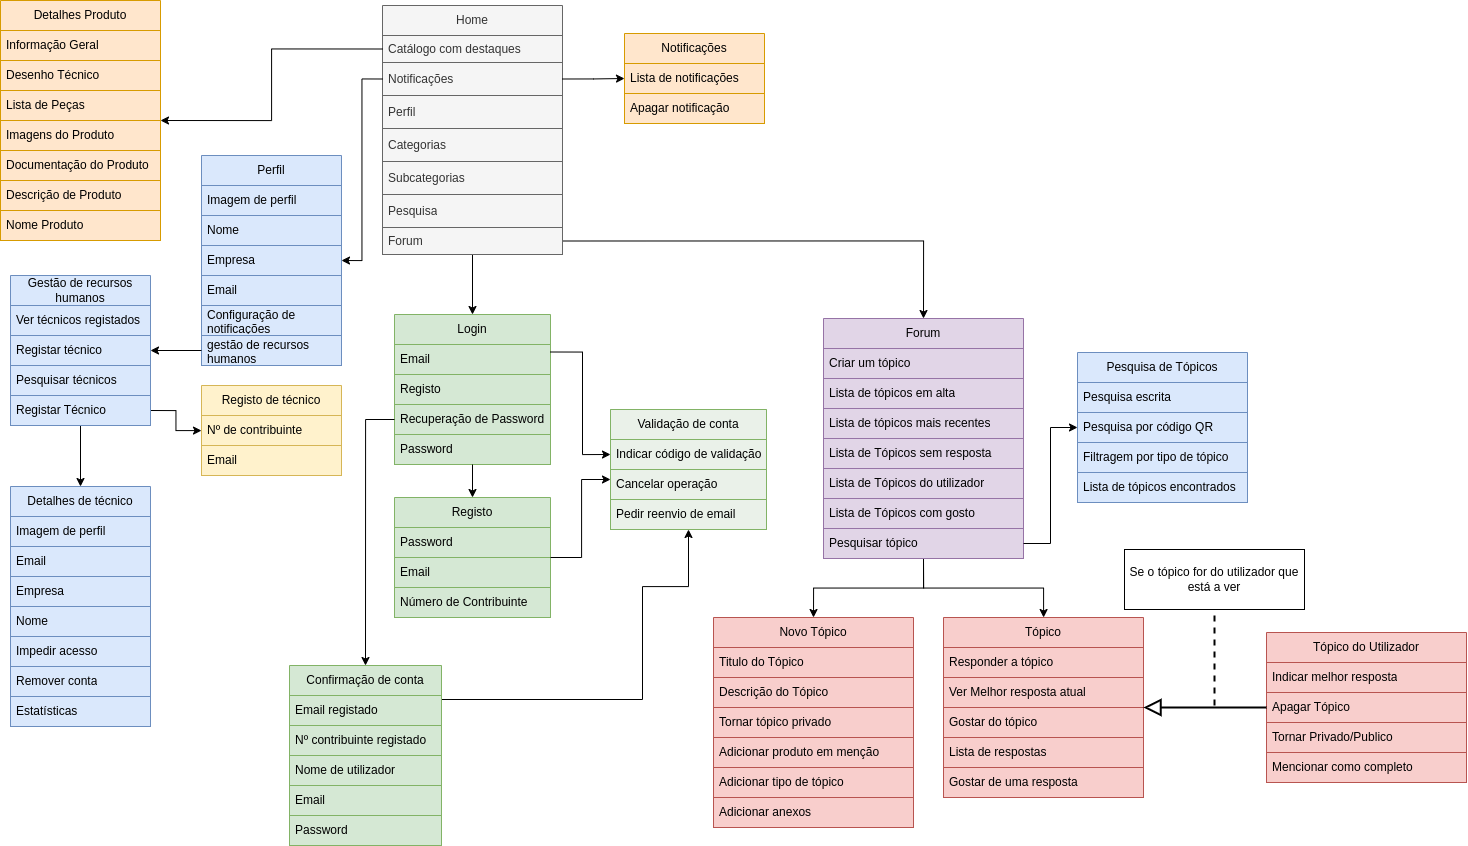
\includegraphics[width=\textwidth]{images/Arquiteturas/diagrama_superficial_de_aplicacao.png}
  \caption{Esquema de organização de páginas do \textit{software}}
  \label{fig:3}
\end{figure}

\newpage

\subsection{Autenticação e página Inicial}

Através deste esquema é possível perceber que do ecrã principal, o utilizador tem acesso ao 
catálogo de produtos e ao fórum, neste pode também realizar o \textit{login} e o \textit{logout} que redirecionam para os respetivos ecrãs.

No ecrã de \textit{login} é necessário o utilizador indicar o número de contribuinte e a \textit{\textit{password}}, neste ele pode também pedir recuperação de \textit{\textit{password}} e/ou redirecionar para o registo onde necessitará de número de contribuinte, \textit{\textit{password}} e \textit{email} para o realizar.

Em caso de o utilizador não possuir a conta ativa, este será encaminhado para o ecrã de validação conta em que deverá indicar o código de validação, cancelar a operação e pedir o reenvio do código de validação.

Em caso de se tratar de um técnico que necessita de confirmar a sua conta, este conseguirá ver as informações registadas, introduzir o seu nome, alterar o seu \textit{email} e \textit{password}.

\begin{figure}[htb]
  \centering
  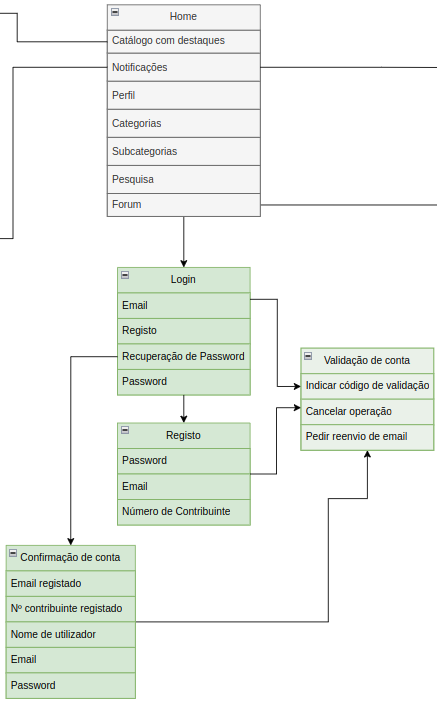
\includegraphics[height=0.9\textwidth]{images/Arquiteturas/superficial_de_app/home_auth.png}
  \caption{Esquema de organização das páginas de autenticação e página inicial}
  \label{fig:4}
\end{figure}

\newpage

\subsection{Fórum}

Através do ecrã inicial o utilizador pode direcionar-se para o ecrã do fórum. Neste ecrã, poderá pesquisar por tópicos, ou então aceder a tópicos em alta, mais recentes ou sem resposta.
O técnico consegue também criar e ver as suos tópicos.

\begin{figure}[htb]
  \centering
  
  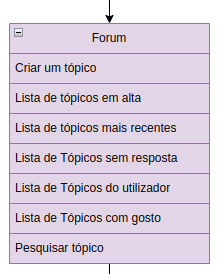
\includegraphics[height=0.4\textwidth]{images/Arquiteturas/superficial_de_app/forum.png}
  \caption{Esquema de organização da página de fórum}
  \label{fig:5}
\end{figure}

\subsection{Criar nova tópico}

Quando o técnico decide criar uma tópico, este tem de indicar o título e a descrição, de seguida poderá indicar se é privado ou não, o tipo de tópico, o produto referente e adicionar anexos.

\begin{figure}[htb]
  \centering
  
  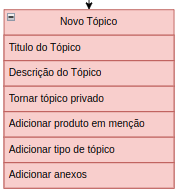
\includegraphics[height=0.3\textwidth]{images/Arquiteturas/superficial_de_app/criar_topico.png}
  \caption{Esquema de organização da página de criação de tópicos}
  \label{fig:6}
\end{figure}

\newpage

\subsection{Detalhes de tópicos}

O técnico pode também ver os detalhes da tópico, responder, 
gostar e gostar de uma resposta.
Caso esta seja do mesmo, este pode indicar a melhor resposta, apagar a tópico, tornar pública ou privada e indicar como completa.

\begin{figure}[htb]
  \centering
  
  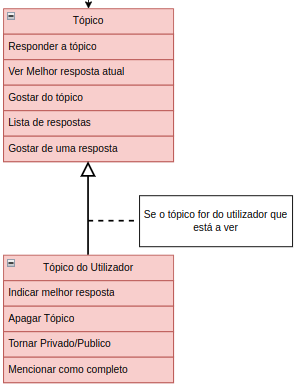
\includegraphics[height=0.55\textwidth]{images/Arquiteturas/superficial_de_app/detalhes_topico.png}
  \caption{Esquema de organização da página de detalhes de tópico}
  \label{fig:7}
\end{figure}

\subsection{Pesquisa de tópicos}

A página de pesquisa permite ao técnico procurar por tópicos específicos tanto por nome como por produto. Para além da pesquisa o utilizador pode também realizar a filtragem dos 
tópicos por tipo e categoria.
\begin{figure}[htb]
  \centering
  
  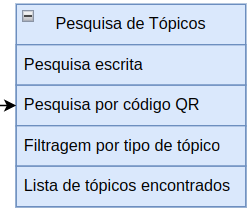
\includegraphics[height=0.3\textwidth]{images/Arquiteturas/superficial_de_app/pesquisa_forum.png}
  \caption{Esquema de organização da página de pesquisa de tópicos}
  \label{fig:8}
\end{figure}

\subsection{Notificações}

A página de notificações permite ao técnico visualizar as suas notificações, assim como também apagar.
\begin{figure}[htb]
  \centering
  
  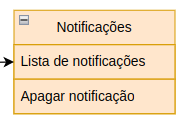
\includegraphics[height=0.2\textwidth]{images/Arquiteturas/superficial_de_app/notificacoes.png}
  \caption{Esquema de organização da página de notificações}
  \label{fig:9}
\end{figure}

\subsection{Perfil}

A página de perfil de técnico permite visualizar as suas informações, assim como alterar 
o seu \textit{email} e configurar as notificações. Caso se trate de uma empresa a visualizar o seu perfil, esta poderá ter acesso à gestão de recursos humanos, para gerir os seus técnicos.
\begin{figure}[htb]
  \centering
  
  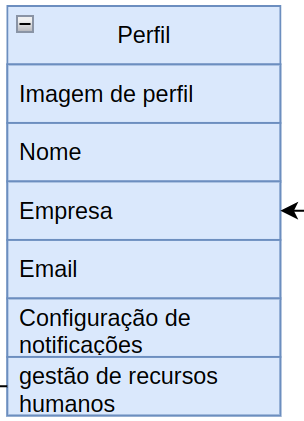
\includegraphics[height=0.35\textwidth]{images/Arquiteturas/superficial_de_app/perfil.png}
  \caption{Esquema de organização da página de perfil}
  \label{fig:10}
\end{figure}

\newpage

\subsection{Gestão de recursos humanos}

A página de gestão de recursos humanos permite à empresa gerir todos os seus técnicos registados e criar contas. Assim que a empresa seleciona um técnico, esta vê o seu perfil, 
com estatísticas.
\begin{figure}[htb]
  \centering
  
  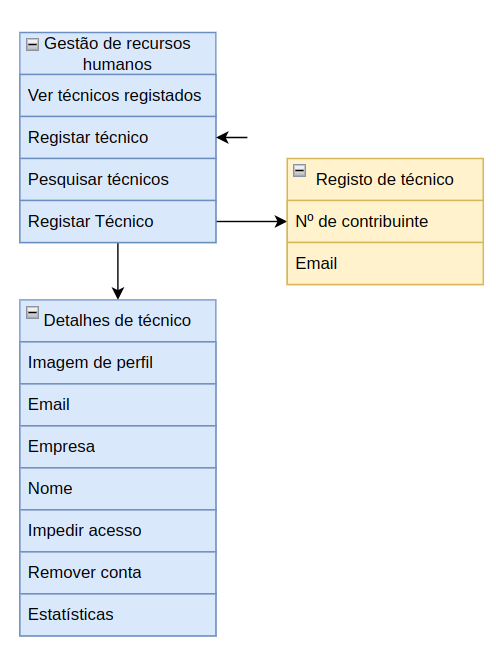
\includegraphics[height=0.7\textwidth]{images/Arquiteturas/superficial_de_app/gestao_recursos_humanos.png}
  \caption{Esquema de organização da página de gestão de recursos humanos}
  \label{fig:11}
\end{figure}

 \newpage

 \section{Histórias de Utilizador}
Antes de desenvolver os casos de uso foram criadas histórias de utilizador para ser possível descrever os objetivos ao realizar uma ação.

% \usepackage{color}
% \usepackage{tabularray}
\definecolor{Concrete}{rgb}{0.952,0.952,0.952}
\begin{longtblr}
[
caption={Tabela de histórias de utilizador},
label={tab:3},
]{
     width = \linewidth,
     colspec = {Q[75]Q[110]Q[700]},
     row{1} = {Concrete},
  row{2} = {Concrete},
  row{8} = {Concrete},
  row{19} = {Concrete},
  row{25} = {Concrete},
  row{30} = {Concrete},
  row{34} = {Concrete},
  row{39} = {Concrete},
  row{43} = {Concrete},
  row{47} = {Concrete},
  column{2} = {c},
  cell{1}{1} = {c},
  cell{2}{2} = {c=2}{0.891\linewidth},
  cell{3}{1} = {c},
  cell{4}{1} = {c},
  cell{5}{1} = {c},
  cell{8}{2} = {c=2}{0.891\linewidth},
  cell{9}{1} = {c},
  cell{10}{1} = {c},
  cell{11}{1} = {c},
  cell{12}{1} = {c},
  cell{13}{1} = {c},
  cell{14}{1} = {c},
  cell{15}{1} = {c},
  cell{16}{1} = {c},
  cell{17}{1} = {c},
  cell{18}{1} = {c},
  cell{19}{2} = {c=2}{0.891\linewidth},
  cell{20}{1} = {c},
  cell{21}{1} = {c},
  cell{22}{1} = {c},
  cell{23}{1} = {c},
  cell{24}{1} = {c},
  cell{25}{2} = {c=2}{0.891\linewidth},
  cell{26}{1} = {c},
  cell{27}{1} = {c},
  cell{28}{1} = {c},
  cell{29}{1} = {c},
  cell{30}{2} = {c=2}{0.891\linewidth},
  cell{31}{1} = {c},
  cell{32}{1} = {c},
  cell{33}{1} = {c},
  cell{34}{2} = {c=2}{0.891\linewidth},
  cell{35}{1} = {c},
  cell{36}{1} = {c},
  cell{37}{1} = {c},
  cell{38}{1} = {c},
  cell{39}{2} = {c=2}{0.891\linewidth},
  cell{40}{1} = {c},
  cell{41}{1} = {c},
  cell{42}{1} = {c},
  cell{43}{2} = {c=2}{0.891\linewidth},
  cell{44}{1} = {c},
  cell{45}{1} = {c},
  cell{46}{1} = {c},
  cell{47}{2} = {c=2}{0.891\linewidth},
  cell{48}{1} = {c},
  cell{49}{1} = {c},
  cell{50}{1} = {c},
  hlines,
  vlines,
}
\#   & Ator                       & Descrição                                                                                                                                                                              \\
     & Autenticação               &                                                                                                                                                                                        \\
US01 & Utilizador                 & Eu como Utilizador, quero conseguir utilizar a aplicação sem realizar o login                                                                                                          \\
US02 & Empresa                    & Eu como Empresa, quero conseguir realizar o registo na aplicação                                                                                                                       \\
US03 & Técnico                    & Eu como Técnico, quero conseguir realizar o login na aplicação utilizando o número de contribuinte e \textit{password}                                                                          \\
US04 & Técnico                    & Eu como Técnico, quero conseguir pedir reenvio de código de ativação de conta caso eu não receba o código                                                                              \\
US05 & Técnico                    & Eu como Técnico, quero conseguir ser identificado como tal na aplicação                                                                                                                \\
     & Fórum                      &                                                                                                                                                                                        \\*
US06 & Técnico                    & Eu como Técnico, quero conseguir acessar ao fórum                                                                                                                                      \\*
US07 & Técnico                    & Eu como Técnico, quero conseguir visualizar os tópicos mais recentes, de forma a conseguir ver os mais falados no dia atual                                                            \\
US08 & Técnico                    & Eu como Técnico, quero conseguir visualizar os tópicos em destaque, de forma a ver quais são mais falados                                                                      \\
US09 & Técnico                    & Eu como Técnico, quero conseguir ver os meus tópicos de forma a conseguir aceder a estes facilmente                                                                                    \\
US10 & Técnico                    & Eu como Técnico, quero conseguir visualizar os tópicos por responder, de forma a conseguir ajudar alguém com maior facilidade                                                          \\
US11 & Técnico                    & Eu como Técnico, quero conseguir visualizar os tópicos privados                                                                                                                        \\
US12 & Técnico                    & Eu como Técnico, quero conseguir realizar filtragem de tópicos por tipo                                                                                \\
US13 & Técnico                    & Eu como Técnico, quero conseguir pesquisar por um tópico relativo a um assunto de forma a obter a solução                                                                              \\
US14 & Técnico                    & Eu como Técnico, quero conseguir pesquisar por um tópico relativo a um produto de forma a encontrar questões comuns a este                                                             \\
US15 & Técnico                    & Eu como Técnico, quero conseguir pesquisar por código QR de um produto de forma a encontrar tópicos referentes ao mesmo mais facilmente                                                 \\
     & Criar Tópico               &                                                                                                                                                                                        \\*
US16 & Técnico                    & Eu como Técnico, quero conseguir criar tópicos de forma a conseguir expor questões                                                                                                     \\*
US17 & Técnico                    & Eu como Técnico, quero conseguir indicar se o meu tópico é publico ou privado, de forma a conseguir respostas de qualquer cliente, ou apenas de técnicos                               \\*
US18 & Técnico                    & Eu como Técnico, quero conseguir indicar o tipo de tópico em que o este se enquadra de forma a facilitar a sua identificação                                                          \\*
US19 & Técnico                    & Eu como Técnico, quero conseguir indicar o produto referente ao tópico para facilitar a identificação do mesmo                                                                         \\*
US20 & Técnico                    & Eu como Técnico, quero conseguir anexar imagens ao tópico de forma a facilitar a comunicação e identificação do problema                                                               \\*
     & Gestão de Tópico           &                                                                                                                                                                                        \\*
US21 & Técnico                    & Eu como Técnico quero conseguir indicar qual a melhor resposta ao meu tópico de forma a facilitar o encontro da solução do problema a outros clientes ou técnicos com o mesmo problema \\*
US22 & Técnico                    & Eu como Técnico quero conseguir indicar que o tópico se encontra finalizado quando o problema está resolvido                                                                           \\
US23 & Técnico                    & Eu como Técnico quero conseguir remover o meu tópico                                                                                                                                   \\
US24 & Técnico                    & Eu como Técnico quero conseguir alterar a visibilidade do meu tópico                                                                                                                   \\
     & Tópicos                    &                                                                                                                                                                                        \\
US25 & Técnico                    & Eu como Técnico, quero conseguir ver todas as respostas a um tópico                                                                                                                    \\
US26 & Técnico                    & Eu como Técnico, quero conseguir gostar de um tópico caso o ache relevante                                                                                                             \\
US27 & Técnico                    & Eu como Técnico, quero conseguir apagar uma resposta minha                                                                                                                             \\
     & Respostas a Tópicos        &                                                                                                                                                                                        \\
US28 & Técnico                    & Eu como Técnico, quero conseguir comentar um tópico de forma a dar a minha resposta                                                                                                    \\
US29 & Técnico                    & Eu como Técnico, quero conseguir responder a um comentário de forma a comunicar                                                                                                        \\
US30 & Técnico                    & Eu como Técnico, quero conseguir anexar imagens ao meu comentário                                                                                                                      \\
US31 & Técnico                    & Eu como Técnico, quero conseguir gostar de um comentário caso ache este relevante                                                                                                      \\
     & Perfil                     &                                                                                                                                                                                        \\*
US32 & Técnico                    & Eu como Técnico quero conseguir alterar o meu \textit{email}                                                                                                                                    \\*
US33 & Técnico                    & Eu como Técnico quero conseguir alterar a minha imagem de perfil                                                                                                                       \\*
US34 & Técnico                    & Eu como Técnico quero conseguir alterar o meu nome                                                                                                                                     \\*
     & Notificações               &                                                                                                                                                                                        \\
US35 & Técnico                    & Eu como Técnico quero conseguir receber notificações por \textit{email} e/ou push de forma a manter-me atualizado das minhas questões                                                           \\
US36 & Técnico                    & Eu como Técnico quero conseguir alterar o tipo de notificação que recebo entre relatório diário e tempo real                                                                           \\
US37 & Técnico                    & Eu como Técnico quero conseguir apagar as minhas notificações de forma a evitar aglomeração                                                                                            \\
     & Gestão de recursos humanos &                                                                                                                                                                                        \\*
US38 & Empresa                    & Eu como Empresa quero conseguir criar conta para os meus técnicos utilizarem o fórum                                                                                                   \\
US39 & Empresa                    & Eu como Empresa quero conseguir impedir acesso a uma conta de técnico                                                                                                                  \\
US40 & Empresa                    & Eu como Empresa quero conseguir remover uma conta de técnico em caso de este já não pertencer à empresa                                                                                
\end{longtblr}

 \newpage

\section{Casos de uso}
Para transformar as histórias de utilizador em ações e especificar todas as reações do sistema com o qual o ator interage foram desenvolvidos casos de uso.

% \usepackage{color}
% \usepackage{tabularray}
\definecolor{Concrete}{rgb}{0.952,0.952,0.952}
\definecolor{Gallery}{rgb}{0.937,0.937,0.937}
\begin{longtblr}
[
caption={Tabela de casos de uso},
label={tab:4},
]
{
  width = \linewidth,
  colspec = {Q[130]Q[81]Q[120]Q[242]Q[375]},
  row{1} = {Concrete},
  row{2} = {Concrete,c},
  row{4} = {Concrete,c},
  row{8} = {Concrete,c},
  row{10} = {Concrete,c},
  row{18} = {Concrete,c},
  row{23} = {Concrete,c},
  row{26} = {Concrete,c},
  row{28} = {Concrete,c},
  row{31} = {Concrete,c},
  column{2} = {c},
  column{3} = {c},
  cell{1}{1} = {c},
  cell{2}{1} = {c=5}{0.936\linewidth},
  cell{4}{1} = {c=5}{0.936\linewidth},
  cell{8}{1} = {c=5}{0.936\linewidth},
  cell{10}{1} = {c=5}{0.936\linewidth},
  cell{18}{1} = {c=5}{0.936\linewidth},
  cell{23}{1} = {c=5}{0.936\linewidth},
  cell{26}{1} = {c=5}{0.936\linewidth},
  cell{28}{1} = {c=5}{0.936\linewidth},
  cell{31}{1} = {c=5}{0.936\linewidth},
  hlines,
  vlines,
}
\#                         & User Story         & Ator       & Nome                                & Descrição                                                   \\
Criar tópico               &                    &            &                                     &                                                             \\
UC 1.0                     & US15               & Técnico    & Criar novo tópico                   & Criação de um novo tópico no fórum                          \\
Pesquisa de tópicos        &                    &            &                                     &                                                             \\
UC 1.1                     & US11               & Técnico    & Pesquisar tópicos específicos       & Pesquisar por tópicos no fórum                              \\
UC 1.1.1                   & US12 e US13        & Técnico    & Pesquisa escrita                    & Pesquisar tópicos por assunto                               \\
UC 1.1.2                   & US14               & Técnico    & Pesquisa por código QR              & Pesquisar tópicos referentes a um produto                   \\
Listagens de tópicos       &                    &            &                                     &                                                             \\
UC 1.2                     & US05               & Técnico    & Ver tópicos                         & Ver listagens de tópicos do fórum                           \\
Detalhes de tópico         &                    &            &                                     &                                                             \\
UC 1.3                     & US08               & Técnico    & Selecionar tópico                   & Ver detalhes de um tópico selecionado                       \\
UC 1.3.1                   & US21               & Técnico    & Finalizar tópico                    & Finalizar um tópico para indicar que está respondido        \\
UC 1.3.2                   & US20               & Técnico    & Selecionar melhor resposta          & Selecionar a melhor resposta do tópico                      \\
UC 1.3.3                   & US22               & Técnico    & Eliminar tópico                     & Eliminar um tópico do fórum                                 \\
UC 1.3.4                   & US23               & Técnico    & Alterar visibilidade do tópico      & Alterar a visibilidade de um tópico entre publico e privado \\
UC 1.3.5                   & US28               & Técnico    & Comentar o tópico                   & Comentar um tópico                                          \\
UC 1.3.6                   & US25               & Técnico    & Gostar de tópico                    & Gostar de um tópico                                         \\
Comentários                &                    &            &                                     &                                                             \\
UC 1.3.7                   & US24               & Técnico    & Ver comentários                     & Ver comentários do tópico                                   \\
UC 1.3.7.1                 & US27               & Técnico    & Apagar comentário                   & Apagar comentário de um tópico                              \\
UC 1.3.7.2                 & US29               & Técnico    & Responder a comentário              & Responder a um comentário de um tópico                      \\
UC 1.3.7.3                 & US31               & Técnico    & Gostar de comentário                & Gostar de um comentário                                     \\
Ativação de conta          &                    &            &                                     &                                                             \\
UC 1.4                     & -                  & Técnico    & Ativação de conta                   & Ativar conta de cliente                                     \\
UC 1.4.1                   & US04               & Técnico    & Pedir reenvio de código de ativação & Pedir reenvio de email de código de ativação                \\
Perfil                     &                    &            &                                     &                                                             \\
UC 1.5                     & US31 - US32 - US33 & Técnico    & Ver Perfil                          & Ver perfil de utilizador                                    \\
Notificações               &                    &            &                                     &                                                             \\
UC1.6                      & US34 e US36        & Técnico    & Ver notificações                    & Ver todas as notificações                                   \\
UC1.7                      & US34 e US35        & Técnico    & Configuração de notificações        & Configurar o modo e tipo de notificações a receber          \\
Gestão de recursos humanos &                    &            &                                     &                                                             \\
UC1.8                      & US37               & Empresa    & Registar Técnico                    & Registar conta de técnico da empresa                        \\
UC1.9                      & US38               & Empresa    & Impedir acesso a técnico            & Registar conta de técnico da empresa                        \\
UC1.10                     & US39               & Empresa    & Remover conta de técnico            & Registar conta de técnico da empresa                        
\end{longtblr}
\newpage

\subsection{Especificação de casos de uso}

Para demonstrar todas as interações entre os atores e o sistema, assim como todas as ações e fluxos possíveis, foram realizadas especificações de casos de uso.

\subsubsection{Especificação de caso de uso de listagem de tópicos}

Através da listagem de tópicos é possível visualizar todas as listagens que o utilizador poderá visualizar, sendo que, o técnico oficial consegue para além destas listagens, ver os seus tópicos e os tópicos privados.

%\definecolor{Concrete}{rgb}{0.952,0.952,0.952}
\begin{longtblr}
[
caption={Tabela de especificação de caso de uso de listagem de tópicos do utilizador},
label={tab:8},
]
{
  width = \linewidth,
  colspec = {Q[225]Q[331]Q[383]},
  row{6} = {Concrete},
  cell{1}{1} = {Concrete},
  cell{1}{2} = {c=2}{0.714\linewidth},
  cell{2}{1} = {Concrete},
  cell{2}{2} = {c=2}{0.714\linewidth},
  cell{3}{1} = {Concrete},
  cell{3}{2} = {c=2}{0.714\linewidth},
  cell{4}{1} = {Concrete},
  cell{4}{2} = {c=2}{0.714\linewidth,c},
  cell{5}{1} = {Concrete},
  cell{5}{2} = {c=2}{0.714\linewidth,c},
  cell{6}{2} = {c},
  cell{6}{3} = {c},
  cell{7}{1} = {r=2}{Concrete},
  cell{9}{1} = {r=2}{Concrete},
  cell{11}{1} = {r=2}{Concrete},
  vlines,
  hline{1-7,9,11,13} = {-}{},
  hline{8,10,12} = {2-3}{},
}
Caso de Uso           & Ver listagem de tópicos                                               &                                  \\
Descrição             & Ver a listagem de tópicos existentes no fórum por diversas categorias &                                  \\
Ator                  & Utilizador                                                            &                                  \\
Pré-condição          & -                                                                     &                                  \\
Pós-condição          & -                                                                     &                                  \\
                      & Ator                                                                  & Sistema                          \\
Fluxo Principal       & 1-Ver tópicos populares                                               &                                  \\
                      &                                                                       & 2-Lista de tópicos populares     \\
Fluxo Alternativo(A1) & 1-Ver tópicos mais recentes                                           &                                  \\
                      &                                                                       & 2-Lista de tópicos mais recentes \\
Fluxo Alternativo(A2) & 1-Ver tópicos por responder                                           &                                  \\
                      &                                                                       & 2-Lista de tópicos por responder 
\end{longtblr}

\definecolor{Concrete}{rgb}{0.952,0.952,0.952}
\begin{longtblr}
[
caption={Tabela de especificação de caso de uso de listagem de tópicos do técnico},
label={tab:5},
]
{
  width = \linewidth,
  colspec = {Q[225]Q[331]Q[383]},
  row{6} = {Concrete},
  cell{1}{1} = {Concrete},
  cell{1}{2} = {c=2}{0.714\linewidth},
  cell{2}{1} = {Concrete},
  cell{2}{2} = {c=2}{0.714\linewidth},
  cell{3}{1} = {Concrete},
  cell{3}{2} = {c=2}{0.714\linewidth},
  cell{4}{1} = {Concrete},
  cell{4}{2} = {c=2}{0.714\linewidth,c},
  cell{5}{1} = {Concrete},
  cell{5}{2} = {c=2}{0.714\linewidth,c},
  cell{6}{2} = {c},
  cell{6}{3} = {c},
  cell{7}{1} = {r=2}{Concrete},
  cell{9}{1} = {r=2}{Concrete},
  cell{11}{1} = {r=2}{Concrete},
  cell{13}{1} = {r=2}{Concrete},
  vlines,
  hline{1-7,9,11,13,15} = {-}{},
  hline{8,10,12,14} = {2-3}{},
}
Caso de Uso           & Ver listagem de tópicos                                               &                                  \\
Descrição             & Ver a listagem de tópicos existentes no fórum por diversas categorias &                                  \\
Ator                  & Técnico                                                            &                                  \\
Pré-condição          & -                                                                     &                                  \\
Pós-condição          & -                                                                     &                                  \\
                      & Ator                                                                  & Sistema                          \\
Fluxo Principal       & 1-Ver tópicos populares                                               &                                  \\
                      &                                                                       & 2-Lista de tópicos populares     \\
Fluxo Alternativo(A1) & 1-Ver tópicos mais recentes                                           &                                  \\
                      &                                                                       & 2-Lista de tópicos mais recentes \\
Fluxo Alternativo(A2) & 1-Ver meus tópicos                                                    &                                  \\
                      &                                                                       & 2-Lista de tópicos do técnico    \\
Fluxo Alternativo(A3) & 1-Ver tópicos por responder                                           &                                  \\
                      &                                                                       & 2-Lista de tópicos por responder 
\end{longtblr}

\newpage

\subsubsection{Especificação de caso de uso de criar novo tópico}

Aquando a criação de um tópico, um técnico poderá realizar diversas ações sendo que obrigatoriamente terá de indicar o título, descrição e tipo de tópico, para além desta informação o técnico poderá anexar imagens, referenciar um produto e indicar a visibilidade.

\definecolor{Concrete}{rgb}{0.952,0.952,0.952}
\begin{longtblr}
[
caption={Tabela de especificação de caso de uso login},
label={tab:6},
]{
 width = \linewidth,
 colspec = {Q[212]Q[360]Q[369]},
 row{6} = {Concrete},
 cell{1}{1} = {Concrete},
 cell{1}{2} = {c=2}{0.725\linewidth},
 cell{2}{1} = {Concrete},
 cell{2}{2} = {c=2}{0.725\linewidth},
 cell{3}{1} = {Concrete},
 cell{3}{2} = {c=2}{0.725\linewidth},
 cell{4}{1} = {Concrete},
 cell{4}{2} = {c=2}{0.725\linewidth},
 cell{5}{1} = {Concrete},
 cell{5}{2} = {c=2}{0.725\linewidth,c},
 cell{6}{2} = {c},
 cell{6}{3} = {c},
 cell{7}{1} = {r=10}{Concrete,c},
 cell{17}{1} = {Concrete},
 cell{18}{1} = {r=6}{Concrete},
 vlines,
 hline{1-7,17-18,24} = {-}{},
 hline{8-16,19-23} = {2-3}{},
}
Caso de Uso      & Criar novo tópico           &                    \\
Descrição       & Criação de um novo tópico no fórum   &                    \\
Ator         & Técnico                &                    \\
Pré-condição     & Clicar em adicionar novo tópico    &                    \\
Pós-condição     & -                   &                    \\
           & Ator                  & Sistema                \\
Fluxo Principal    & 1-Indicar o título do tópico      &                    \\
           & 2-Indicar a descrição do tópico    &                    \\
           & 3-Indicar se o tópico é privado    &                    \\
           & 4-Indicar o tipo do tópico       &                    \\
           & 5-Indicar o produto referido no tópico &                    \\
           & 6-Adicionar imagens de anexo      &                    \\
           & 7-Confirmar a criação do tópico    &                    \\
           &                    & 8-Verificar se titulo está inserido  \\
           &                    & 9-Verificar se descrição está inserida \\
           &                    & 10-Inserir novo tópico no fórum    \\
Fluxo Alternativo(A1) & 1-Cancelar a criação do tópico     &                    \\
Fluxo Alternativo(A2) & 1-Indicar o título do tópico      &                    \\*
           & 2-Indicar se o tópico é privado    &                    \\*
           & 3-Confirmar a criação do tópico    &                    \\*
           &                    & 4-Verificar se titulo está inserido  \\*
           &                    & 5-Verificar se descrição está inserida \\*
           &                    & 6-Erro descrição em falta     
\end{longtblr}

\newpage

\subsubsection{Especificação de caso de uso de pesquisar tópicos por escrito}

Assim que um técnico deseje pesquisar por um assunto específico de tópico este poderá realizar uma pesquisa escrita onde conseguirá realizar filtragem por tipo e categoria de tópico.

% \usepackage{color}
% \usepackage{tabularray}
\definecolor{Concrete}{rgb}{0.952,0.952,0.952}
\begin{longtblr}
[
caption={Tabela de especificação de caso de uso de pesquisa por escrito},
label={tab:6},
]{
  width = \linewidth,
  colspec = {Q[190]Q[217]Q[533]},
  row{6} = {Concrete},
  cell{1}{1} = {Concrete},
  cell{1}{2} = {c=2}{0.702\linewidth},
  cell{2}{1} = {Concrete},
  cell{2}{2} = {c=2}{0.702\linewidth},
  cell{3}{1} = {Concrete},
  cell{3}{2} = {c=2}{0.702\linewidth},
  cell{4}{1} = {Concrete},
  cell{4}{2} = {c=2}{0.702\linewidth},
  cell{5}{1} = {Concrete},
  cell{5}{2} = {c=2}{0.702\linewidth,c},
  cell{6}{2} = {c},
  cell{6}{3} = {c},
  cell{7}{1} = {r=4}{Concrete},
  cell{11}{1} = {r=2}{Concrete},
  vlines,
  hline{1-7,11,13} = {-}{},
  hline{8-10,12} = {2-3}{},
}
Caso de Uso           & Pesquisa por escrita           &                                            \\
Descrição             & Pesquisar por tópicos no fórum &                                            \\
Ator                  & Utilizador                     &                                            \\
Pré-condição          & Selecionar pesquisa de fórum   &                                            \\
Pós-condição          & -                              &                                            \\
                      & Ator                           & Sistema                                    \\
Fluxo Principal       & 1-Pesquisar assunto            &                                            \\
                      &                                & 2-Lista de tópicos do assunto              \\
                      & 3-Filtrar por tipo             &                                            \\
                      &                                & 3-Filtragem de tópicos do assunto por tipo \\
Fluxo Alternativo(A1) & 1-Pesquisar assunto            &                                            \\
                      &                                & 2-Lista de tópicos do assunto              
\end{longtblr}


\subsubsection{Especificação de caso de uso de ver finalizar tópico}

Quando um técnico encontra-se satisfeito com a solução do problema este poderá indicar que o tópico está finalizado, o que é sinalizado para outros técnicos.

% \usepackage{color}
% \usepackage{tabularray}
\definecolor{Concrete}{rgb}{0.952,0.952,0.952}
\begin{table}[htb]
\centering
\label{tab:8}
\caption{Tabela de especificação de caso de uso de finalizar tópico}
\begin{tblr}{
  width = \linewidth,
  colspec = {Q[254]Q[319]Q[365]},
  row{6} = {Concrete},
  cell{1}{1} = {Concrete},
  cell{1}{2} = {c=2}{0.683\linewidth},
  cell{2}{1} = {Concrete},
  cell{2}{2} = {c=2}{0.683\linewidth},
  cell{3}{1} = {Concrete},
  cell{3}{2} = {c=2}{0.683\linewidth},
  cell{4}{1} = {Concrete},
  cell{4}{2} = {c=2}{0.683\linewidth},
  cell{5}{1} = {Concrete},
  cell{5}{2} = {c=2}{0.683\linewidth},
  cell{6}{2} = {c},
  cell{6}{3} = {c},
  cell{7}{1} = {r=2}{Concrete},
  cell{9}{1} = {Concrete},
  cell{9}{2} = {c},
  cell{9}{3} = {c},
  vlines,
  hline{1-7,9-10} = {-}{},
  hline{8} = {2-3}{},
}
Caso de Uso           & Finalizar tópico                                     &                                  \\
Descrição             & Finalizar um tópico para indicar que está respondido &                                  \\
Ator                  & Técnico                                              &                                  \\
Pré-condição          & Clicar no tópico desejado                            &                                  \\
Pós-condição          & Alterar tópico para finalizado                       &                                  \\
                      & Ator                                                 & Sistema                          \\
Fluxo Principal       & 1-Clicar em finalizar tópico                         &                                  \\
                      &                                                      & 2-Alterar tópico para finalizado \\
Fluxo Alternativo(A1) & -                                                    & -                                
\end{tblr}
\end{table}

\newpage

\subsubsection{Especificação de caso de uso de selecionar melhor resposta}

Sempre que o técnico encontrar uma resposta no seu tópico que se destaca na solução da sua questão, este poderá colocar esta resposta como a melhor resposta do tópico. Caso já exista uma melhor resposta, esta automáticamente é removida e a nova é colocada como melhor resposta.

% \usepackage{color}
% \usepackage{tabularray}
\definecolor{Concrete}{rgb}{0.952,0.952,0.952}
\begin{table}[htb]
\centering
\label{tab:9}
\caption{Tabela de especificação de caso de uso de selecionar melhor resposta}
\begin{tblr}{
 width = \linewidth,
 colspec = {Q[181]Q[235]Q[525]},
 row{6} = {Concrete},
 cell{1}{1} = {Concrete},
 cell{1}{2} = {c=2}{0.76\linewidth},
 cell{2}{1} = {Concrete},
 cell{2}{2} = {c=2}{0.76\linewidth},
 cell{3}{1} = {Concrete},
 cell{3}{2} = {c=2}{0.76\linewidth},
 cell{4}{1} = {Concrete},
 cell{4}{2} = {c=2}{0.76\linewidth},
 cell{5}{1} = {Concrete},
 cell{5}{2} = {c=2}{0.76\linewidth},
 cell{6}{2} = {c},
 cell{6}{3} = {c},
 cell{7}{1} = {r=3}{Concrete},
 cell{10}{1} = {r=4}{Concrete},
 cell{14}{1} = {r=4}{Concrete},
 vlines,
 hline{1-7,10,14,18} = {-}{},
 hline{8-9,11-13,15-17} = {2-3}{},
}
Caso de Uso      & Selecionar melhor resposta       &                                 \\
Descrição       & Selecionar a melhor resposta do tópico &                                 \\
Ator         & Técnico                 &                                 \\
Pré-condição     & Clicar no tópico desejado        &                                 \\
Pós-condição     & Alterar a resposta para melhor resposta &                                 \\
           & Ator                  & Sistema                             \\
Fluxo Principal    & 1-Clicar em melhor resposta       &                                 \\
           &                     & 2-Verificar se já existe uma melhor resposta - Não        \\
           &                     & 3- Colocar a resposta como melhor resposta do tópico       \\
Fluxo Alternativo(A1) & 1-Clicar em melhor resposta       &                                 \\
           &                     & 2-Verificar se já existe uma melhor resposta - Sim        \\
           &                     & 3- Verificar se a resposta existente é a mesma selecionada - Não \\
           &                     & 4-Alterar melhor resposta                    \\
Fluxo Alternativo(A2) & 1-Clicar em melhor resposta       &                                 \\
           &                     & 2-Verificar se já existe uma melhor resposta - Sim        \\
           &                     & 3- Verificar se a resposta existente é a mesma selecionada - Sim \\
           &                     & 4-Remover melhor resposta                    
\end{tblr}
\end{table}

\newpage

\subsubsection{Especificação de caso de uso de eliminar tópico}

O técnico sempre que desejar poderá eliminar o tópico, o que permite remover do fórum e não volta a ser apresentado.

% \usepackage{color}
% \usepackage{tabularray}
\definecolor{Concrete}{rgb}{0.952,0.952,0.952}
\begin{table}[htb]
\centering
\label{tab:12}
\caption{Tabela de especificação do caso de uso de eliminar tópico}
\begin{tblr}{
  width = \linewidth,
  colspec = {Q[290]Q[371]Q[273]},
  row{6} = {Concrete},
  cell{1}{1} = {Concrete},
  cell{1}{2} = {c=2}{0.644\linewidth},
  cell{2}{1} = {Concrete},
  cell{2}{2} = {c=2}{0.644\linewidth},
  cell{3}{1} = {Concrete},
  cell{3}{2} = {c=2}{0.644\linewidth},
  cell{4}{1} = {Concrete},
  cell{4}{2} = {c=2}{0.644\linewidth},
  cell{5}{1} = {Concrete},
  cell{5}{2} = {c=2}{0.644\linewidth},
  cell{6}{2} = {c},
  cell{6}{3} = {c},
  cell{7}{1} = {r=2}{Concrete},
  cell{9}{1} = {Concrete},
  cell{9}{2} = {c},
  cell{9}{3} = {c},
  vlines,
  hline{1-7,9-10} = {-}{},
  hline{8} = {2-3}{},
}
Caso de Uso           & Eliminar tópico             &                    \\
Descrição             & Eliminar um tópico do fórum &                    \\
Ator                  & Técnico                     &                    \\
Pré-condição          & Clicar no tópico desejado   &                    \\
Pós-condição          & Remoção do tópico           &                    \\
                      & Ator                        & Sistema            \\
Fluxo Principal       & 1-Clicar em remover tópico  &                    \\
                      &                             & 3-Remover o tópico \\
Fluxo Alternativo(A1) & -                           & -                  
\end{tblr}
\end{table}

\subsubsection{Especificação de caso de uso de alterar visibilidade de um tópico}

Quando um técnico pública um tópico este pode desejar alterar a sua visibilidade para apenas técnicos oficiais ou todos os técnicos.

% \usepackage{color}
% \usepackage{tabularray}
\definecolor{Concrete}{rgb}{0.952,0.952,0.952}
\begin{table}[htb]
\centering
\label{tab:11}
\caption{Tabela de especificação de caso de uso de alteração de visibilidade de um tópico}
\begin{tblr}{
 width = \linewidth,
 colspec = {Q[242]Q[344]Q[354]},
 row{6} = {Concrete},
 cell{1}{1} = {Concrete},
 cell{1}{2} = {c=2}{0.698\linewidth},
 cell{2}{1} = {Concrete},
 cell{2}{2} = {c=2}{0.698\linewidth},
 cell{3}{1} = {Concrete},
 cell{3}{2} = {c=2}{0.698\linewidth},
 cell{4}{1} = {Concrete},
 cell{4}{2} = {c=2}{0.698\linewidth},
 cell{5}{1} = {Concrete},
 cell{5}{2} = {c=2}{0.698\linewidth},
 cell{6}{2} = {c},
 cell{6}{3} = {c},
 cell{7}{1} = {r=2}{Concrete},
 cell{9}{1} = {Concrete},
 cell{9}{2} = {c},
 cell{9}{3} = {c},
 vlines,
 hline{1-7,9-10} = {-}{},
 hline{8} = {2-3}{},
}
Caso de Uso      & Alterar visibilidade do tópico               &                  \\
Descrição       & Alterar a visibilidade de um tópico entre público e privado &                  \\
Ator         & Técnico                           &                  \\
Pré-condição     & Clicar no tópico desejado                  &                  \\
Pós-condição     & Alterar visibilidade do tópico               &                  \\
           & Ator                            & Sistema              \\
Fluxo Principal    & 1-Clicar em alterar visibilidade              &                  \\
           &                               & 2-Inverter visibilidade do tópico \\
Fluxo Alternativo(A1) & -                              & -                 
\end{tblr}
\end{table}

\newpage

\subsubsection{Especificação de caso de uso gostar de um tópico}

O técnico sempre que encontra um tópico que identifica como útil, este poderá colocar \textit{like} o que gera destaque.

% \usepackage{color}
% \usepackage{tabularray}
\definecolor{Concrete}{rgb}{0.952,0.952,0.952}
\begin{table}[htb]
\centering
\label{tab:12}
\caption{Tabela de especificação de caso de uso de gostar de um tópico}
\begin{tblr}{
  width = \linewidth,
  colspec = {Q[260]Q[221]Q[458]},
  row{6} = {Concrete},
  cell{1}{1} = {Concrete},
  cell{1}{2} = {c=2}{0.679\linewidth},
  cell{2}{1} = {Concrete},
  cell{2}{2} = {c=2}{0.679\linewidth},
  cell{3}{1} = {Concrete},
  cell{3}{2} = {c=2}{0.679\linewidth},
  cell{4}{1} = {Concrete},
  cell{4}{2} = {c=2}{0.679\linewidth},
  cell{5}{1} = {Concrete},
  cell{5}{2} = {c=2}{0.679\linewidth},
  cell{6}{2} = {c},
  cell{6}{3} = {c},
  cell{7}{1} = {r=3}{Concrete},
  cell{10}{1} = {r=3}{Concrete},
  vlines,
  hline{1-7,10,13} = {-}{},
  hline{8-9,11-12} = {2-3}{},
}
Caso de Uso           & Gostar do tópico          &                                        \\
Descrição             & Gostar de um tópico       &                                        \\
Ator                  & Técnico                   &                                        \\
Pré-condição          & Clicar no tópico desejado &                                        \\
Pós-condição          & Alterar gostos do tópico  &                                        \\
                      & Ator                      & Sistema                                \\
Fluxo Principal       & 1-Clicar em gosto         &                                        \\
                      &                           & 2-Verificar se o gosto já existe - Não \\
                      &                           & 3-Acrescentar gosto ao tópico          \\
Fluxo Alternativo(A1) & 1-Clicar em gosto         &                                        \\
                      &                           & 2-Verificar se o gosto já existe - Sim \\
                      &                           & 3-Remover gosto do tópico              
\end{tblr}
\end{table}


\subsubsection{Especificação de caso de uso gostar de um comentário}

Sempre que um técnico identificar um comentário como útil este poderá colcoar \textit{like} o que gera destaque.

% \usepackage{color}
% \usepackage{tabularray}
\definecolor{Concrete}{rgb}{0.952,0.952,0.952}
\begin{table}[htb]
\centering
\label{tab:13}
\caption{Tabela de especificação de caso de uso de gostar de comentário}
\begin{tblr}{
  width = \linewidth,
  colspec = {Q[260]Q[221]Q[458]},
  row{6} = {Concrete},
  cell{1}{1} = {Concrete},
  cell{1}{2} = {c=2}{0.679\linewidth},
  cell{2}{1} = {Concrete},
  cell{2}{2} = {c=2}{0.679\linewidth},
  cell{3}{1} = {Concrete},
  cell{3}{2} = {c=2}{0.679\linewidth},
  cell{4}{1} = {Concrete},
  cell{4}{2} = {c=2}{0.679\linewidth},
  cell{5}{1} = {Concrete},
  cell{5}{2} = {c=2}{0.679\linewidth,c},
  cell{6}{2} = {c},
  cell{6}{3} = {c},
  cell{7}{1} = {r=3}{Concrete},
  cell{10}{1} = {r=3}{Concrete},
  vlines,
  hline{1-7,10,13} = {-}{},
  hline{8-9,11-12} = {2-3}{},
}
Caso de Uso           & Gostar de comentário      &                                        \\
Descrição             & Gostar de um comentário   &                                        \\
Ator                  & Técnico                   &                                        \\
Pré-condição          & Clicar no tópico desejado &                                        \\
Pós-condição          & -                         &                                        \\
                      & Ator                      & Sistema                                \\
Fluxo Principal       & 1-Clicar em gosto         &                                        \\
                      &                           & 2-Verificar se o gosto já existe - Não \\
                      &                           & 3-Acrescentar gosto ao comentário      \\
Fluxo Alternativo(A1) & 1-Clicar em gosto         &                                        \\
                      &                           & 2-Verificar se o gosto já existe - Sim \\
                      &                           & 3-Remover gosto do tópico              
\end{tblr}
\end{table}

\newpage

\subsubsection{Especificação de caso de uso de comentar tópico}

Sempre que um técnico encontra um tópico sobre uma questão que poderá ajudar, este consegue responder através de um comentário, onde este também poderá adicionar imagens.

% \usepackage{color}
% \usepackage{tabularray}
\definecolor{Concrete}{rgb}{0.952,0.952,0.952}
\begin{table}[htb]
\centering
\label{tab:14}
\caption{Tabela de especificação de caso de uso de comentar um tópico}
\begin{tblr}{
 width = \linewidth,
 colspec = {Q[225]Q[348]Q[367]},
 row{6} = {Concrete},
 cell{1}{1} = {Concrete},
 cell{1}{2} = {c=2}{0.715\linewidth},
 cell{2}{1} = {Concrete},
 cell{2}{2} = {c=2}{0.715\linewidth},
 cell{3}{1} = {Concrete},
 cell{3}{2} = {c=2}{0.715\linewidth},
 cell{4}{1} = {Concrete},
 cell{4}{2} = {c=2}{0.715\linewidth},
 cell{5}{1} = {Concrete},
 cell{5}{2} = {c=2}{0.715\linewidth},
 cell{6}{2} = {c},
 cell{6}{3} = {c},
 cell{7}{1} = {r=4}{Concrete},
 cell{11}{1} = {r=3}{Concrete},
 cell{14}{1} = {Concrete},
 vlines,
 hline{1-7,11,14-15} = {-}{},
 hline{8-10,12-13} = {2-3}{},
}
Caso de Uso      & Comentar o tópico         &                   \\
Descrição       & Comentar um tópico        &                   \\
Ator         & Técnico              &                   \\
Pré-condição     & Clicar no tópico desejado     &                   \\
Pós-condição     & Inserir a resposta no tópico   &                   \\
           & Ator               & Sistema               \\
Fluxo Principal    & 1-Indicar a descrição da resposta &                   \\
           & 2-Anexar Imagem          &                   \\
           & 3-Confirmar a resposta      &                   \\
           &                  & 4-Inserir novo comentário no tópico \\
Fluxo Alternativo(A1) & 1-Indicar a descrição da resposta &                   \\
           & 2-Confirmar a resposta      &                   \\
           &                  & 3-Inserir novo comentário no tópico \\
Fluxo Alternativo(A2) & 1-Cancelar a criação do tópico  &                   
\end{tblr}
\end{table}

\newpage

\subsubsection{Especificação de caso de uso ativar conta}

O técnico para ativar a sua conta deverá introduzir o código de ativação correto, caso contrário não será possível ativar.

% \usepackage{color}
% \usepackage{tabularray}
\definecolor{Concrete}{rgb}{0.952,0.952,0.952}
\begin{longtblr}
  [
  caption={Tabela de especificação de caso de uso ativação de conta},
  label={tab:15},
  ]{
  width = \linewidth,
  colspec = {Q[219]Q[300]Q[419]},
  row{6} = {Concrete},
  cell{1}{1} = {Concrete},
  cell{1}{2} = {c=2}{0.719\linewidth},
  cell{2}{1} = {Concrete},
  cell{2}{2} = {c=2}{0.719\linewidth},
  cell{3}{1} = {Concrete},
  cell{3}{2} = {c=2}{0.719\linewidth},
  cell{4}{1} = {Concrete},
  cell{4}{2} = {c=2}{0.719\linewidth,c},
  cell{5}{1} = {Concrete},
  cell{5}{2} = {c=2}{0.719\linewidth,c},
  cell{6}{2} = {c},
  cell{6}{3} = {c},
  cell{7}{1} = {r=4}{Concrete},
  cell{11}{1} = {Concrete},
  cell{12}{1} = {r=4}{Concrete},
  vlines,
  hline{1-7,11-12,16} = {-}{},
  hline{8-10,13-15} = {2-3}{},
}
Caso de Uso           & Ativar conta                  &                                           \\
Descrição             & Ativar conta de aplicação     &                                           \\
Ator                  & Técnico                       &                                           \\
Pré-condição          & -                             &                                           \\
Pós-condição          & -                             &                                           \\
                      & Ator                          & Sistema                                   \\
Fluxo Principal       & 1-Inserir código de validação &                                           \\
                      & 2-Validar conta               &                                           \\
                      &                               & 3-Verificar se o código está correto- Sim \\
                      &                               & 4-Validar conta                           \\
Fluxo Alternativo(A1) & 1-Cancelar Ativação de conta  &                                           \\
Fluxo Alternativo(A2) & 1-Inserir código de validação &                                           \\
                      & 2-Validar conta               &                                           \\
                      &                               & 3-Verificar se o código está correto- Não \\
                      &                               & 4-Código de valdiação incorreto           
\end{longtblr}

\newpage

\subsubsection{Especificação de caso de uso configurar notificações}

As notificações da aplicação poderão ser personalizadas, o que possibilita escolher entre \textit{email}, \textit{push} e ambos,
para além destas configurações, é também possível personalizar o tipo de notificação para cada método, seja relatório diário de todas as notificações ou notificações em tempo real.

% \usepackage{color}
% \usepackage{tabularray}
\definecolor{Concrete}{rgb}{0.952,0.952,0.952}
\begin{table}[htb]
\centering
\label{tab:16}
\caption{Tabela de especificação de caso de uso de configuração de notificações}
\begin{tblr}{
 width = \linewidth,
 colspec = {Q[258]Q[575]Q[108]},
 row{6} = {Concrete},
 cell{1}{1} = {Concrete},
 cell{1}{2} = {c=2}{0.682\linewidth},
 cell{2}{1} = {Concrete},
 cell{2}{2} = {c=2}{0.682\linewidth},
 cell{3}{1} = {Concrete},
 cell{3}{2} = {c=2}{0.682\linewidth},
 cell{4}{1} = {Concrete},
 cell{4}{2} = {c=2}{0.682\linewidth},
 cell{5}{1} = {Concrete},
 cell{5}{2} = {c=2}{0.682\linewidth},
 cell{6}{2} = {c},
 cell{6}{3} = {c},
 cell{7}{1} = {r=2}{Concrete},
 cell{9}{1} = {Concrete},
 vlines,
 hline{1-7,9-10} = {-}{},
 hline{8} = {2-3}{},
}
Caso de Uso      & Configuração de notificações           &     \\
Descrição       & Configuração de notificações do técnico     &     \\
Ator         & Técnico                     &     \\
Pré-condição     & -                        &     \\
Pós-condição     & -                        &     \\
           & Ator                       & Sistema \\
Fluxo Principal    & 1-Indicar preferência de receção de notificações &     \\
           & 2-Indicar tipo de receção de notificações    &     \\
Fluxo Alternativo(A1) & 1-Ver notificações                &     
\end{tblr}
\end{table}

\subsubsection{Especificação de caso de uso registar técnico}

Sempre que uma empresa deseja realizar o registo de técnicos em seu nome, esta poderá indicar o nºcontribuinte e \textit{email}, com isto, este receberá um \textit{email} para confirmar o registo de conta.

% \usepackage{color}
% \usepackage{tabularray}
\definecolor{Concrete}{rgb}{0.952,0.952,0.952}
\begin{table}[htb]
\centering
\label{tab:17}
\caption{Tabela de especificação de caso de uso de registar técnico}
\begin{tblr}{
  width = \linewidth,
  colspec = {Q[331]Q[454]Q[142]},
  row{6} = {Concrete},
  cell{1}{1} = {Concrete},
  cell{1}{2} = {c=2}{0.627\linewidth},
  cell{2}{1} = {Concrete},
  cell{2}{2} = {c=2}{0.627\linewidth},
  cell{3}{1} = {Concrete},
  cell{3}{2} = {c=2}{0.627\linewidth},
  cell{4}{1} = {Concrete},
  cell{4}{2} = {c=2}{0.627\linewidth},
  cell{5}{1} = {Concrete},
  cell{5}{2} = {c=2}{0.627\linewidth},
  cell{6}{2} = {c},
  cell{6}{3} = {c},
  cell{7}{1} = {r=3}{Concrete},
  cell{10}{1} = {Concrete},
  cell{10}{2} = {c},
  cell{10}{3} = {c},
  vlines,
  hline{1-7,10-11} = {-}{},
  hline{8-9} = {2-3}{},
}
Caso de Uso           & Registar técnico                     &                    \\
Descrição             & Registar conta de técnico da empresa &                    \\
Ator                  & Empresa                              &                    \\
Pré-condição          & -                                    &                    \\
Pós-condição          & -                                    &                    \\
                      & Ator                                 & Sistema            \\
Fluxo Principal       & 1-Indicar o nºcontribuinte           &                    \\
                      & 2-Indicar \textit{email}                      &                    \\
                      &                                      & 3-Registar técnico \\
Fluxo Alternativo(A1) & -                                    & -                  
\end{tblr}
\end{table}


% \subsubsection{Especificação de caso de uso responder a comentário}

% O técnico poderá manter uma conversa com outros técnicos através da resposta a outros comentários, 
% a qual poderá também incluir imagens.

% % \usepackage{color}
% \usepackage{tabularray}
\definecolor{Concrete}{rgb}{0.952,0.952,0.952}
\begin{table}[htb]
\centering
\label{tab:18}
\caption{Tabela de especificação de caso de uso de responder a comentário}
\begin{tblr}{
  width = \linewidth,
  colspec = {Q[229]Q[381]Q[333]},
  row{6} = {Concrete},
  cell{1}{1} = {Concrete},
  cell{1}{2} = {c=2}{0.714\linewidth},
  cell{2}{1} = {Concrete},
  cell{2}{2} = {c=2}{0.714\linewidth},
  cell{3}{1} = {Concrete},
  cell{3}{2} = {c=2}{0.714\linewidth},
  cell{4}{1} = {Concrete},
  cell{4}{2} = {c=2}{0.714\linewidth},
  cell{5}{1} = {Concrete},
  cell{5}{2} = {c=2}{0.714\linewidth},
  cell{6}{2} = {c},
  cell{6}{3} = {c},
  cell{7}{1} = {r=2}{Concrete},
  cell{9}{1} = {Concrete},
  cell{9}{2} = {c},
  cell{9}{3} = {c},
  vlines,
  hline{1-7,9-10} = {-}{},
  hline{8} = {2-3}{},
}
Caso de Uso           & Responder a comentário                 &                                 \\
Descrição             & Responder a um comentário de um tópico &                                 \\
Ator                  & Técnico                                &                                 \\
Pré-condição          & Clicar no tópico desejado              &                                 \\
Pós-condição          & Novo comentário                        &                                 \\
                      & Ator                                   & Sistema                         \\
Fluxo Principal       & 1-Clicar em responder a comentário     &                                 \\
                      &                                        & 2-Inserir resposta a comentário \\
Fluxo Alternativo(A1) & -                                      & -                               
\end{tblr}
\end{table}

%---------------------------------------------------------------------------------

% \subsubsection{Especificação de caso de uso registo}

% A empresa deverá realizar o registo utilizando o número de contribuinte, \textit{email} e \textit{password}. Após este 
% registo, a Motorline validará o registo e de seguida um \textit{email} é enviado para confirmar o registo na app.

% % \usepackage{color}
% \usepackage{tabularray}
\definecolor{Concrete}{rgb}{0.952,0.952,0.952}
\begin{table}[htb]
\centering
\label{tab:21}
\caption{Tabela de especificação de caso de uso de registo}
\begin{tblr}{
 width = \linewidth,
 colspec = {Q[267]Q[348]Q[323]},
 row{6} = {Concrete},
 cell{1}{1} = {Concrete},
 cell{1}{2} = {c=2}{0.671\linewidth},
 cell{2}{1} = {Concrete},
 cell{2}{2} = {c=2}{0.671\linewidth},
 cell{3}{1} = {Concrete},
 cell{3}{2} = {c=2}{0.671\linewidth},
 cell{4}{1} = {Concrete},
 cell{4}{2} = {c=2}{0.671\linewidth},
 cell{5}{1} = {Concrete},
 cell{5}{2} = {c=2}{0.671\linewidth},
 cell{6}{2} = {c},
 cell{6}{3} = {c},
 cell{7}{1} = {r=7}{Concrete},
 cell{14}{1} = {Concrete},
 vlines,
 hline{1-7,14-15} = {-}{},
 hline{8-13} = {2-3}{},
}
Caso de Uso      & Registo de cliente ou técnico       &            \\
Descrição       & Registo de cliente ou técnico na aplicação &            \\
Ator         & Cliente                  &            \\
Pré-condição     & -                     &            \\
Pós-condição     & Email de verificação de código       &            \\
           & Ator                    & Sistema        \\
Fluxo Principal    & 1-Indicar Nº Contribuinte         &            \\
           & 2-Indicar nome de empresa         &            \\
           & 3-Indicar Email              &            \\
           & 4-Password                 &            \\
           & 5-Confirmação Password           &            \\
           &                      & 6-Verificar Registo  \\
           &                      & 7-Mensagem de Sucesso \\
Fluxo Alternativo(A1) & 1-Cancelar Registo             &            
\end{tblr}
\end{table}

%---------------------------------------------------------------------------------

% \subsubsection{Especificação de caso de uso pedir reenvio de código de verificação}

% O técnico poderá aquando a validação da sua conta pedir o reenvio de um novo código de validação em caso 
% de algum imprevisto.

% % \usepackage{color}
% \usepackage{tabularray}
\definecolor{Concrete}{rgb}{0.952,0.952,0.952}
\begin{table}[htb]
\centering
\begin{tblr}{
  width = \linewidth,
  colspec = {Q[223]Q[356]Q[362]},
  row{6} = {Concrete},
  cell{1}{1} = {Concrete},
  cell{1}{2} = {c=2}{0.706\linewidth},
  cell{2}{1} = {Concrete},
  cell{2}{2} = {c=2}{0.706\linewidth},
  cell{3}{1} = {Concrete},
  cell{3}{2} = {c=2}{0.706\linewidth},
  cell{4}{1} = {Concrete},
  cell{4}{2} = {c=2}{0.706\linewidth,c},
  cell{5}{1} = {Concrete},
  cell{5}{2} = {c=2}{0.706\linewidth},
  cell{6}{2} = {c},
  cell{6}{3} = {c},
  cell{7}{1} = {r=3}{Concrete},
  cell{10}{1} = {Concrete},
  cell{10}{2} = {c},
  cell{10}{3} = {c},
  vlines,
  hline{1-7,10-11} = {-}{},
  hline{8-9} = {2-3}{},
}
Caso de Uso           & Pedir reenvio de código de ativação          &                                 \\
Descrição             & Pedir reenvio de \textit{email} de código de ativação &                                 \\
Ator                  & Técnico                                      &                                 \\
Pré-condição          & -                                            &                                 \\
Pós-condição          & Email de verificação de código               &                                 \\
                      & Ator                                         & Sistema                         \\
Fluxo Principal       & 1-Pedir novo código de ativação              &                                 \\
                      &                                              & 2-Gerar novo código de ativação \\
                      &                                              & 3-Enviar novo \textit{email}             \\
Fluxo Alternativo(A1) & -                                            & -                               
\end{tblr}
\end{table}

%---------------------------------------------------------------------------------

% \subsubsection{Especificação de caso de uso confirmar conta}

% Sempre que uma conta de técnico é criada, este deverá proceder à confirmação da conta, nesta confirmação
% o técnico tem de inidicar o seu nome de utilizador, poderá alterar o \textit{email} de registo e terá de indicar a
% \textit{password} e confirmação de \textit{password}, procedendo depois à ativação da conta.

% % \usepackage{color}
% \usepackage{tabularray}
\definecolor{Concrete}{rgb}{0.952,0.952,0.952}
\begin{table}[htb]
\centering
\begin{tblr}{
 width = \linewidth,
 colspec = {Q[258]Q[429]Q[254]},
 row{6} = {Concrete},
 cell{1}{1} = {Concrete},
 cell{1}{2} = {c=2}{0.683\linewidth},
 cell{2}{1} = {Concrete},
 cell{2}{2} = {c=2}{0.683\linewidth},
 cell{3}{1} = {Concrete},
 cell{3}{2} = {c=2}{0.683\linewidth},
 cell{4}{1} = {Concrete},
 cell{4}{2} = {c=2}{0.683\linewidth,c},
 cell{5}{1} = {Concrete},
 cell{5}{2} = {c=2}{0.683\linewidth,c},
 cell{6}{2} = {c},
 cell{6}{3} = {c},
 cell{7}{1} = {r=6}{Concrete},
 cell{13}{1} = {Concrete},
 vlines,
 hline{1-7,13-14} = {-}{},
 hline{8-12} = {2-3}{},
}
Caso de Uso      & Confirmar conta          &            \\
Descrição       & Confirmar conta de técnico    &            \\
Ator         & Técnico              &            \\
Pré-condição     & -                 &            \\
Pós-condição     & -                 &            \\
           & Ator               & Sistema        \\
Fluxo Principal    & 1-Inserir nome de utilizador   &            \\
           & 2-Indicar Password        &            \\
           & 3-Indicar Confirmação de \textit{password} &            \\
           &                  & 4-Verificar se registo \\
           &                  & 5-Conta registada   \\
           &                  & 6-Validar conta    \\
Fluxo Alternativo(A1) & 1-Cancelar Ativação de conta   &            
\end{tblr}
\end{table}

%---------------------------------------------------------------------------------

% \subsubsection{Especificação de caso de uso ver perfil}

% Sempre que um técnico desejar alterar alguma informação sua, este poderá se dirigir ao seu perfil onde 
% consegue alterar o seu \textit{email} e imagem de perfil.

% % \usepackage{color}
% \usepackage{tabularray}
\definecolor{Concrete}{rgb}{0.952,0.952,0.952}
\begin{table}[htb]
\centering
\begin{tblr}{
 width = \linewidth,
 colspec = {Q[252]Q[310]Q[379]},
 row{6} = {Concrete},
 cell{1}{1} = {Concrete},
 cell{1}{2} = {c=2}{0.689\linewidth},
 cell{2}{1} = {Concrete},
 cell{2}{2} = {c=2}{0.689\linewidth},
 cell{3}{1} = {Concrete},
 cell{3}{2} = {c=2}{0.689\linewidth},
 cell{4}{1} = {Concrete},
 cell{4}{2} = {c=2}{0.689\linewidth},
 cell{5}{1} = {Concrete},
 cell{5}{2} = {c=2}{0.689\linewidth},
 cell{6}{2} = {c},
 cell{6}{3} = {c},
 cell{7}{1} = {r=2}{Concrete},
 cell{9}{1} = {r=2}{Concrete},
 vlines,
 hline{1-7,9,11} = {-}{},
 hline{8,10} = {2-3}{},
}
Caso de Uso      & Ver perfil         &                 \\
Descrição       & Ver perfil do técnico   &                 \\
Ator         & Técnico          &                 \\
Pré-condição     & -             &                 \\
Pós-condição     & -             &                 \\
           & Ator            & Sistema             \\
Fluxo Principal    & 1-Alterar \textit{email}      &                 \\
           &              & 2-Alteração de \textit{email}      \\
Fluxo Alternativo(A1) & 1-Alterar imagem de perfil &                 \\
           &              & 2-Alteração de imagem de perfil 
\end{tblr}
\end{table}

%---------------------------------------------------------------------------------

% \subsubsection{Especificação de caso de uso ver notificações}

% Sempre que um técnico desejar ver todas as suas notificações este poderá ver esta listagem, 
% conseguindo também apagar notificações que já não deseja ver.

% % \usepackage{color}
% \usepackage{tabularray}
\definecolor{Concrete}{rgb}{0.952,0.952,0.952}
\begin{table}[htb]
\centering
\begin{tblr}{
  width = \linewidth,
  colspec = {Q[287]Q[285]Q[363]},
  row{6} = {Concrete},
  cell{1}{1} = {Concrete},
  cell{1}{2} = {c=2}{0.647\linewidth},
  cell{2}{1} = {Concrete},
  cell{2}{2} = {c=2}{0.647\linewidth},
  cell{3}{1} = {Concrete},
  cell{3}{2} = {c=2}{0.647\linewidth},
  cell{4}{1} = {Concrete},
  cell{4}{2} = {c=2}{0.647\linewidth},
  cell{5}{1} = {Concrete},
  cell{5}{2} = {c=2}{0.647\linewidth},
  cell{6}{2} = {c},
  cell{6}{3} = {c},
  cell{7}{1} = {r=2}{Concrete},
  cell{9}{1} = {r=4}{Concrete},
  vlines,
  hline{1-7,9,13} = {-}{},
  hline{8,10-12} = {2-3}{},
}
Caso de Uso           & Ver Notificações            &                            \\
Descrição             & Ver notificações do técnico &                            \\
Ator                  & Técnico                     &                            \\
Pré-condição          & -                           &                            \\
Pós-condição          & -                           &                            \\
                      & Ator                        & Sistema                    \\
Fluxo Principal       & 1-Ver notificações          &                            \\
                      &                             & 2-Listagem de notificações \\
Fluxo Alternativo(A1) & 1-Ver notificações          &                            \\
                      &                             & 2-Listagem de notificações \\
                      & 3-Apagar notificação        &                            \\
                      &                             & 4-Eliminar notificação     
\end{tblr}
\end{table}

%---------------------------------------------------------------------------------

% \subsubsection{Especificação de caso de uso apagar comentário}

% Sempre que o técnico cria um comentário este tem a possibilidade de o remover a qualquer momento que 
% desejar.

% % \usepackage{color}
% \usepackage{tabularray}
\definecolor{Concrete}{rgb}{0.952,0.952,0.952}
\begin{table}[htb]
\centering
\label{tab:17}
\caption{Tabela de especificação de caso de uso de apagar comentário}
\begin{tblr}{
 width = \linewidth,
 colspec = {Q[271]Q[394]Q[273]},
 row{6} = {Concrete},
 cell{1}{1} = {Concrete},
 cell{1}{2} = {c=2}{0.667\linewidth},
 cell{2}{1} = {Concrete},
 cell{2}{2} = {c=2}{0.667\linewidth},
 cell{3}{1} = {Concrete},
 cell{3}{2} = {c=2}{0.667\linewidth},
 cell{4}{1} = {Concrete},
 cell{4}{2} = {c=2}{0.667\linewidth},
 cell{5}{1} = {Concrete},
 cell{5}{2} = {c=2}{0.667\linewidth},
 cell{6}{2} = {c},
 cell{6}{3} = {c},
 cell{7}{1} = {r=2}{Concrete},
 cell{9}{1} = {Concrete},
 cell{9}{2} = {c},
 cell{9}{3} = {c},
 vlines,
 hline{1-7,9-10} = {-}{},
 hline{8} = {2-3}{},
}
Caso de Uso      & Apagar comentário       &           \\
Descrição       & Apagar comentário de um tópico &           \\
Ator         & Técnico            &           \\
Pré-condição     & Clicar no tópico desejado   &           \\
Pós-condição     & Comentário apagado       &           \\
           & Ator              & Sistema       \\
Fluxo Principal    & 1-Clicar em apagar comentário &           \\
           &                & 2-Apagar comentário \\
Fluxo Alternativo(A1) & -               & -          
\end{tblr}
\end{table}

%---------------------------------------------------------------------------------

% \subsubsection{Especificação de caso de uso login}

% O técnico deverá realizar o login utilizando o número de contribuinte e \textit{password}.

% % \usepackage{color}
% \usepackage{tabularray}
\definecolor{Concrete}{rgb}{0.952,0.952,0.952}
\begin{longtblr}
  [
  caption={Tabela de especificação de caso de uso criação de novo tópico},
  label={tab:5},
  ]{
    width = \linewidth,
    colspec = {Q[262]Q[373]Q[306]},
    row{6} = {Concrete},
    cell{1}{1} = {Concrete},
    cell{1}{2} = {c=2}{0.679\linewidth},
    cell{2}{1} = {Concrete},
    cell{2}{2} = {c=2}{0.679\linewidth},
    cell{3}{1} = {Concrete},
    cell{3}{2} = {c=2}{0.679\linewidth},
    cell{4}{1} = {Concrete},
    cell{4}{2} = {c=2}{0.679\linewidth},
    cell{5}{1} = {Concrete},
    cell{5}{2} = {c=2}{0.679\linewidth},
    cell{6}{2} = {c},
    cell{6}{3} = {c},
    cell{7}{1} = {r=4}{Concrete},
    cell{11}{1} = {Concrete},
    cell{12}{1} = {Concrete},
    cell{13}{1} = {r=4}{Concrete},
    vlines,
    hline{1-7,11-13,17} = {-}{},
    hline{8-10,14-16} = {2-3}{},
  }
  Caso de Uso           & Login                            &                          \\
  Descrição             & Iniciar sessão na aplicação      &                          \\
  Ator                  & Técnico                          &                          \\
  Pré-condição          & Código de verificação confirmado &                          \\
  Pós-condição          & Home Screen                      &                          \\
                        & Ator                             & Sistema                  \\
  Fluxo Principal       & 1-Indicar Nº Contribuinte        &                          \\
                        & 2-Indicar Password               &                          \\
                        &                                  & 3-Verificar Login        \\
                        &                                  & 4-Devolver Sessão        \\
  Fluxo Alternativo(A1) & 1-Clicar em não iniciar sessão   &                          \\
  Fluxo Alternativo(A2) & 1-Cancelar Login                 &                          \\
  Fluxo Alternativo(A3) & 1-Indicar Nº Contribuinte        &                          \\
                        & 2-Indicar Password               &                          \\
                        &                                  & 3-Verificar Login        \\
                        &                                  & 4-Erro conta não ativada 
\end{longtblr}

%---------------------------------------------------------------------------------

%\subsubsection{Especificação de caso de uso de pesquisar tópicos por código QR}

%Assim que um utilizador deseje pesquisar por tópicos relativos a um produto, este poderá utilizar 
%o código QR do mesmo, conseguindo também realizar uma pesquisa por escrito.  

%% \usepackage{color}
% \usepackage{tabularray}
\definecolor{Concrete}{rgb}{0.952,0.952,0.952}
\begin{longtblr}
[
caption={Tabela de especificação de caso de uso de pesquisa por código QR},
label={tab:7},
]{
 width = \linewidth,
 colspec = {Q[175]Q[219]Q[546]},
 row{6} = {Concrete},
 cell{1}{1} = {Concrete},
 cell{1}{2} = {c=2}{0.74\linewidth},
 cell{2}{1} = {Concrete},
 cell{2}{2} = {c=2}{0.74\linewidth},
 cell{3}{1} = {Concrete},
 cell{3}{2} = {c=2}{0.74\linewidth},
 cell{4}{1} = {Concrete},
 cell{4}{2} = {c=2}{0.74\linewidth},
 cell{5}{1} = {Concrete},
 cell{5}{2} = {c=2}{0.74\linewidth,c},
 cell{6}{2} = {c},
 cell{6}{3} = {c},
 cell{7}{1} = {r=6}{Concrete},
 cell{13}{1} = {r=4}{Concrete},
 vlines,
 hline{1-7,13,17} = {-}{},
 hline{8-12,14-16} = {2-3}{},
}
Caso de Uso      & Pesquisa por código QR            &                            \\
Descrição       & Pesquisar por tópicos no fórum por código QR &                            \\
Ator         & Utilizador                  &                            \\
Pré-condição     & Selecionar pesquisa de fórum         &                            \\
Pós-condição     & -                      &                            \\
           & Ator                     & Sistema                        \\
Fluxo Principal    & 1-Pesquisar por código QR          &                            \\
           &                       & 2-Lista de tópicos do produto             \\
           & 2-Pesquisar assunto             &                            \\
           &                       & 3-Filtragem de tópicos do produto por assunto     \\
           & 4-Filtrar por tipo              &                            \\
           &                       & 5-Filtragem de tópicos do produto por assunto e tópico \\
Fluxo Alternativo(A1) & 1-Pesquisar por código QR          &                            \\
           &                       & 2-Lista de tópicos do produto             \\
           & 2-Pesquisar assunto             &                            \\
           &                       & 3-Filtragem de tópicos do produto por assunto     
\end{longtblr}

%\newpage

 \newpage

 
\subsection{Diagramas de casos de uso}
Para ser possível visualizar graficamente todas as ações que os 
atores conseguem realizar e para melhorar a comunicação com as 
partes interessadas do projeto, foram desenvolvidos diagramas de 
casos de uso.

\subsubsection{Casos de uso Fórum}
Na imagem representada abaixo (Figura~\ref{fig:12}), é possível 
visualizar o diagrama de casos de uso para o fórum.
Neste, o técnico poderá ver as listagens de tópicos em destaque e tópicos mais recentes. Caso seja um técnico oficial terá acesso aos tópicos privados e os seus tópicos.
O técnico poderá também pesquisar por tópicos, dos quais ele terá a possibilidade de selecionar um para visualizar. 
O técnico conseguirá, além disso, criar um novo tópico, onde se dirigirá para a criação de tópicos. Aqui, o técnico será obrigado a inserir um título, descrição e tipo do tópico para o criar, 
mas poderá inserir imagens e indicar produto referente.
Para finalizar a criação o técnico conseguirá confirmar ou cancelar o processo. 

\begin{figure}[htb]
    \centering
    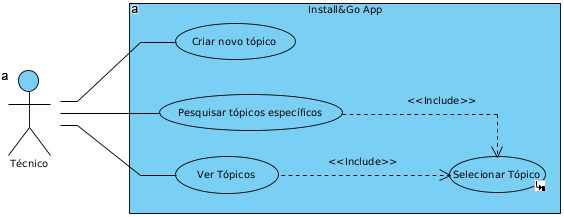
\includegraphics[width=0.6\textwidth]{images/diagramas/casos_de_uso/use_case_forum.png}
    \caption{Diagrama de casos de uso de fórum}
    \label{fig:12}
\end{figure}

\subsubsection{Casos de uso de pesquisar tópicos}

O técnico poderá realizar a pesquisa por tópicos específicos, 
esta será ser realizada por escrito onde indica o assunto a pesquisar e poderá ser filtrada.

O técnico terá também a possibilidade de pesquisar por código QR de produto, uma vez que, o servidor da Motorline esteja desenvolvido para tal.

\begin{figure}[htb]
    \centering
    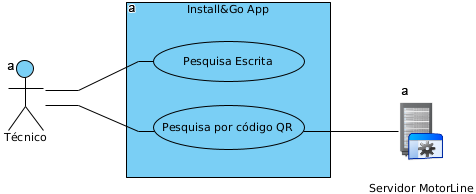
\includegraphics[width=0.6\textwidth]{images/diagramas/casos_de_uso/use_case_forum_search.png}
    \caption{Diagrama de casos de uso de pesquisa de tópicos}
    \label{fig:13}
\end{figure}

\subsubsection{Casos de uso ver detalhes de tópico}

Assim que um técnico seleciona um tópico, é movido para os 
detalhes, onde consegue visualizar os detalhes, responder e, caso seja o seu tópico, consegue finalizar, selecionar a melhor resposta, remover a melhor resposta, eliminar e alterar a visibilidade do tópico.

\begin{figure}[htb]
    \centering
    
    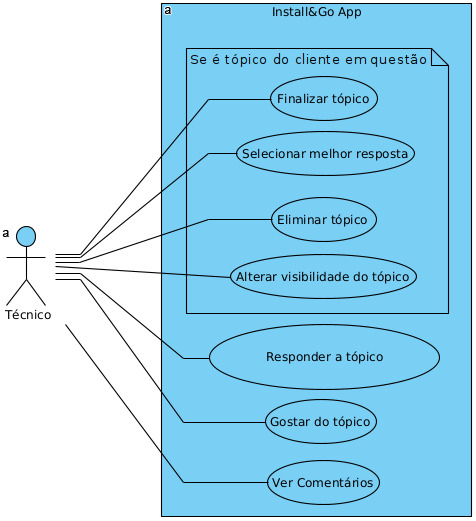
\includegraphics[width=0.5\textwidth]{images/diagramas/casos_de_uso/use_case_topic_details.png}
    \caption{Diagrama de casos de uso de detalhes de tópico}
    \label{fig:14}
\end{figure}

\subsubsection{Casos de uso ver comentários}

O técnico quando decide visualizar os comentários consegue responder e gostar de uma resposta ou comentário, caso este seja seu ainda o consegue apagar.

\begin{figure}[htb]
    \centering
    
    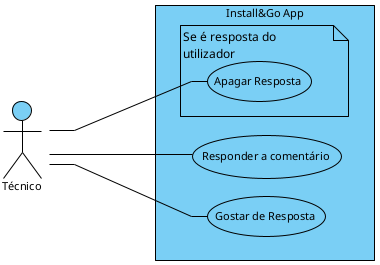
\includegraphics[width=0.5\textwidth]{images/diagramas/casos_de_uso/use_case_topic_comments.png}
    \caption{Diagrama de casos de uso de ver comentários}
    \label{fig:15}
\end{figure}

\subsubsection{Casos de uso ativação de conta}

Assim que uma conta é confirmada, um \textit{email} de ativação é enviado para técnico e esta deverá ser ativada.
Para isto, o código deverá ser indicado pelo técnico para se proceder à ativação da conta. Este, poderá em caso de necessidade, pedir o reenvio do código de ativação, o qual será gerado novamente e reenviado.

\begin{figure}[htb]
    \centering
    
    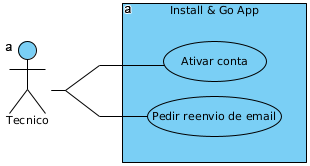
\includegraphics[width=0.5\textwidth]{images/diagramas/casos_de_uso/use_case_account_validation.png}
    \caption{Diagrama de casos de uso de ativação de conta}
    \label{fig:16}
\end{figure}

\subsubsection{Casos de uso perfil}

Sempre que o técnico desejar alterar alguma informação, este poderá alterar o seu nome, \textit{email} e imagem de perfil.

\begin{figure}[htb]
    \centering
    
    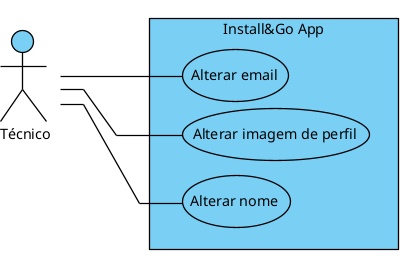
\includegraphics[width=0.5\textwidth]{images/diagramas/casos_de_uso/use_case_perfil.png}
    \caption{Diagrama de casos de uso de perfil}
    \label{fig:17}
\end{figure}

\newpage

\subsubsection{Casos de uso notificações}

Sempre que o técnico desejar ver as suas notificações, poderá seleciona-las, também dispõe da possibilidade de alterar a configuração das notificações, para apenas as receber por \textit{email} ou push, ou então, ambas. Terá também a possibilidade de personalizar cada método, para receber um relatório diário de notificações ou então, notificações em tempo real.

\begin{figure}[htb]
    \centering
    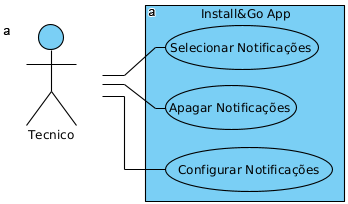
\includegraphics[width=0.5\textwidth]{images/diagramas/casos_de_uso/use_case_notificacoes.png}
    \caption{Diagrama de casos de notificações}
    \label{fig:18}
\end{figure}

\subsubsection{Casos de uso gestão de recursos humanos}

Uma empresa poderá registar contas para os seus técnicos no seu nome, com a indicação do \textit{email} e nºcontribuinte. Esta poderá também impedir acesso a estas contas ou remover completamente a conta da aplicação.

\begin{figure}[htb]
    \centering
    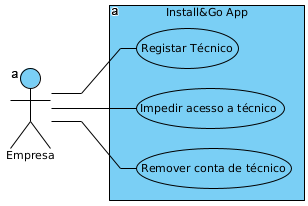
\includegraphics[width=0.5\textwidth]{images/diagramas/casos_de_uso/use_case_rec_humanos.png}
    \caption{Diagrama de casos de uso de recursos humanos}
    \label{fig:19}
\end{figure}

 \newpage

 \section{Diagrama Entidade Relação}

O software Install\&Go é suportado por uma base de dados relacional esquematizada de acordo com as necessidades do projeto. Para garantir que os tipos dos atributos se encontram corretos, foram criados novos tipos, já para simular a criação de \textit{id's} do tipo \textit{uuid} foi criado um \textit{stored procedure} o que resulta na tabela de cor verde na Figura\ref{fig:20}. Encontra-se no documento de anexos, no anexo 17, uma versão em maiores dimensões da Figura~\ref*{fig:20}.


\begin{figure}[htb]
  \centering
  
  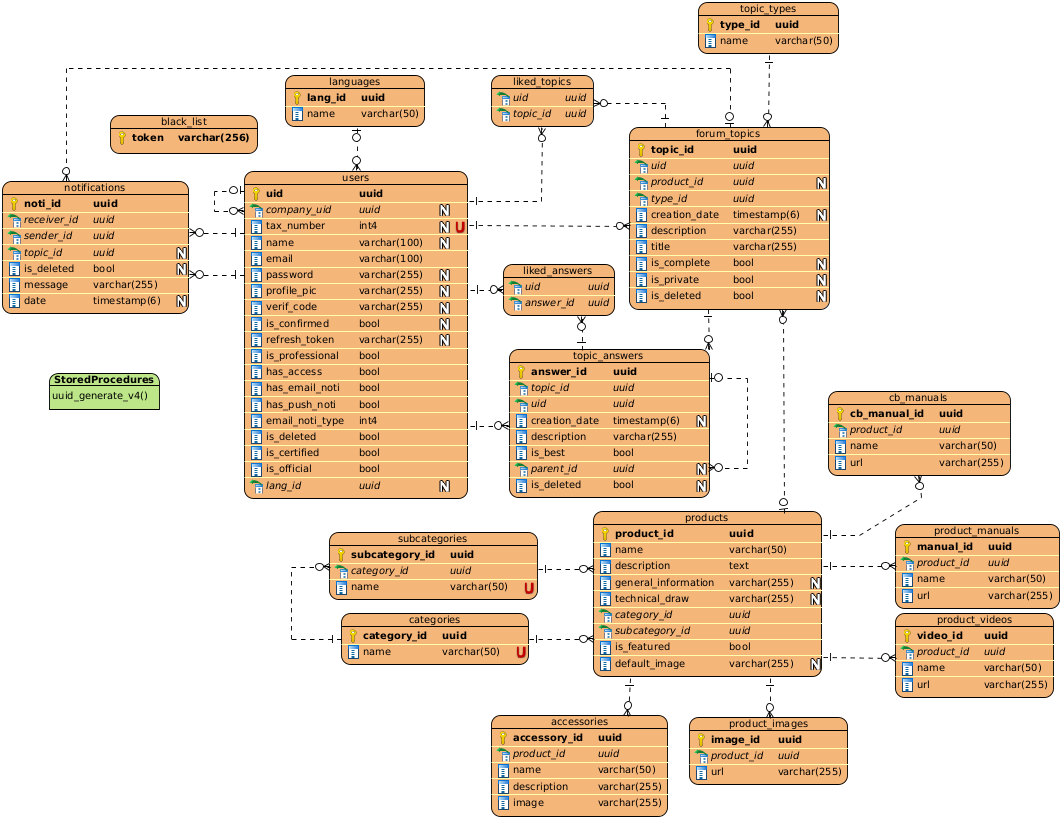
\includegraphics[width=\textwidth]{images/diagramas/diagrama_bd.png}
  \caption{Diagrama Entidade Relação base de dados Install\&Go}
  \label{fig:20}
\end{figure}

\newpage

\subsection{Escolha de diagrama de entidade relação}
Durante o desenvolvimento do diagrama de entidade relação, surgiu 
a opção de separar as empresas dos seus técnicos em duas tabelas como 
exemplificado na Figura~\ref{fig:21}. Neste sempre que se
deseja, por exemplo, obter o utilizador que criou um tópico é necessário
verificar se o \textit{uid} contido é de uma empresa ou de um técnico e apenas de seguida se obter o utilizador que criou o tópico, sendo este um exemplo entre os demais do mesmo tipo. Tendo em conta este problema foi decido optar pelo diagrama da Figura~\ref{fig:20}. Encontra-se no documento de anexos, no anexo 18, uma versão em maiores dimensões da Figura~\ref*{fig:21}.


\begin{figure}[htb]
  \centering
  
  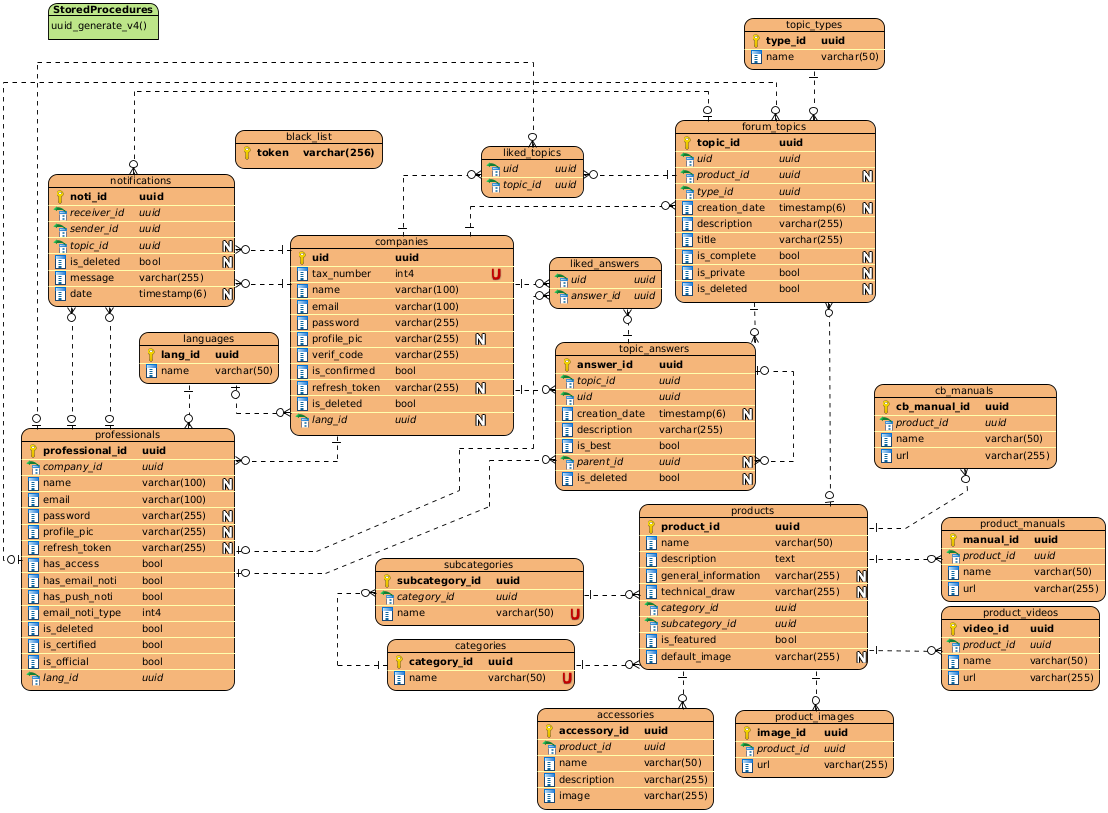
\includegraphics[width=\textwidth]{images/diagramas/diagrama_bd_alt.png}
  \caption{Diagrama Entidade Relação alternativo}
  \label{fig:21}
\end{figure}

\newpage

\subsection{Dicionário de termos}

Com intuito de alcançar o propósito de cada tabela e atributo 
foi criado um dicionário de termos para a base de dados(Tabela~\ref{tab:18}).

\definecolor{Concrete}{rgb}{0.952,0.952,0.952}
\begin{longtblr}
[
caption={Dicionário de termos da base de dados},
label={tab:22},
]{
  width = \linewidth,
  colspec = {Q[220]Q[292]Q[240]Q[215]},
  row{1} = {Concrete},
  column{1} = {c},
  cell{2}{1} = {r=19}{},
  cell{2}{2} = {r=19}{},
  cell{22}{1} = {r=2}{},
  cell{22}{2} = {r=2}{},
  cell{24}{1} = {r=2}{},
  cell{24}{2} = {r=2}{},
  cell{26}{1} = {r=2}{},
  cell{26}{2} = {r=2}{},
  cell{28}{1} = {r=7}{},
  cell{28}{2} = {r=7}{},
  cell{35}{1} = {r=10}{},
  cell{35}{2} = {r=10}{},
  cell{45}{1} = {r=8}{},
  cell{45}{2} = {r=8}{},
  cell{53}{1} = {r=2}{},
  cell{53}{2} = {r=2}{},
  cell{55}{1} = {r=3}{},
  cell{55}{2} = {r=3}{},
  cell{58}{1} = {r=4}{},
  cell{58}{2} = {r=4}{},
  cell{62}{1} = {r=8}{},
  cell{62}{2} = {r=8}{},
  cell{70}{1} = {r=4}{},
  cell{70}{2} = {r=4}{},
  cell{74}{1} = {r=4}{},
  cell{74}{2} = {r=4}{},
  vlines,
  hline{1-2,21-22,24,26,28,35,45,53,55,58,62,70,74,78} = {-}{},
  hline{3-20,23,25,27,29-34,36-44,46-52,54,56-57,59-61,63-69,71-73,75-77} = {3-4}{},
}
Tabela           & Descrição                                                                            & Atributos            & Descrição                                           \\
users            & Tabela encarregue de guardar todos os dados referentes aos utilizadores da aplicação & uid                  & Id do utilizador                                    \\
                 &                                                                                      & company\_id          & Id da empresa referente ao técnico                  \\
                 &                                                                                      & n\_contribuinte      & Número de contribuinte do utilizador                \\
                 &                                                                                      & name                 & Nome do utilizador                                  \\
                 &                                                                                      & email                & Email do utilizador                                 \\
                 &                                                                                      & password             & Password do utilizador                              \\
                 &                                                                                      & profile\_pic         & Imagem de perfil do utilizador                      \\
                 &                                                                                      & verif\_code          & Código de verificação do utilizador                 \\
                 &                                                                                      & is\_confirmed        & Verificação de se o código está confirmado          \\
                 &                                                                                      & refresh\_token       & Token de refresh                                    \\
                 &                                                                                      & is\_professional     & verificação se é profissional                       \\
                 &                                                                                      & has\_access          & verificação se tem acesso à conta                   \\
                 &                                                                                      & has\_email\_noti     & verificação se ativou notificações de email         \\
                 &                                                                                      & has\_push\_noti      & verificação se ativou notificações push             \\
                 &                                                                                      & email\_noti\_type    & tipo de notificação de email                        \\
                 &                                                                                      & push\_noti\_type     & tipo de notificação push                            \\
                 &                                                                                      & is\_deleted          & verificação se a conta se encontra apagada          \\
                 &                                                                                      & is\_certified        & verificação se é um técnico certificado             \\
                 &                                                                                      & is\_official         & verificação se é um técnico oficial                 \\
black\_list      & Tabela que guarda os tokens a bloquear                                               & token                & Token a bloquear                                    \\
liked\_topics    & Tabela encarregue de guardar todos os tópicos que foram gostados pelo utilizador     & uid                  & Id do utilizador                                    \\
                 &                                                                                      & topic\_id            & Id do tópico                                        \\
liked\_answers   & Tabela encarregue de guardar todas as respostas que receberam gosto do utilizador    & uid                  & Id do utilizador                                    \\
                 &                                                                                      & answer\_id           & Id da resposta                                      \\
topic\_types     & Tabela encarregue de guardar os tipos de tópico existentes                           & type\_id             & Id do tipo de tópico                                \\
                 &                                                                                      & name                 & nome do tipo de tópico                              \\
notifications    & Tabela encarregue de guardar todas as notificações do técnico                        & noti\_id             & Id da notificação                                   \\
                 &                                                                                      & receiver\_id         & Recetor da notificação                              \\
                 &                                                                                      & sender\_id           & Emissor da notificação                              \\
                 &                                                                                      & topic\_id            & Id do tópico em caso de estar referente a um tópico \\
                 &                                                                                      & is\_deleted          & verificação se a notificação está apagada           \\
                 &                                                                                      & message              & mensagem da notificação                             \\
                 &                                                                                      & date                 & data de emissão da notificação                      \\
forum\_topics    & Tabela encarregue de guardar todos os tópicos existentes na aplicação                & topic\_id            & Id do tópico                                        \\
                 &                                                                                      & uid                  & Id do dono do tópico                                \\
                 &                                                                                      & product\_id          & Produto referente ao tópico                         \\
                 &                                                                                      & tiype\_id            & Id do tipo referente ao tópico                      \\
                 &                                                                                      & creation\_date       & Data de criação do tópico                           \\
                 &                                                                                      & description          & Descrição do tópico                                 \\
                 &                                                                                      & title                & Titulo do tópico                                    \\
                 &                                                                                      & is\_complete         & Verificação se o tópico está finalizado             \\
                 &                                                                                      & is\_private          & Verificação se o tópico é privado                   \\
                 &                                                                                      & is\_deleted          & Verificação se o tópico está apagado                \\
topic\_answers   & Tabela encarregue de guardar todas as respostas a um tópico                          & answer\_id           & Id da resposta                                      \\
                 &                                                                                      & topic\_id            & Id do tópico                                        \\
                 &                                                                                      & uid                  & Id do dono da resposta                              \\
                 &                                                                                      & creation\_date       & Data de criação da resposta                         \\
                 &                                                                                      & description          & Descrição da resposta                               \\
                 &                                                                                      & is\_best             & Verificação se é a melhor resposta                  \\
                 &                                                                                      & parent\_id           & Id da resposta pai                                  \\
                 &                                                                                      & is\_deleted          & Verificação se o topico se encontra apagado         \\
categories       & Tabela encarregue de guardar todas as categorias de produtos existentes              & category\_id         & Id da categoria                                     \\
                 &                                                                                      & name                 & Nome da categoria                                   \\
subcategories    & Tabela encarregue de guardar as subcategorias de produtos existentes                 & subcategory\_id      & Id da subcategoria                                  \\*
                 &                                                                                      & category\_id         & Id da categoria                                     \\*
                 &                                                                                      & name                 & Nome da subcategoria                                \\*
cb\_manuals      & Tabela encarregue de guardar os manuais de utilização das placas de controlo         & cb\_manual\_id       & Id do manual                                        \\
                 &                                                                                      & product\_id          & Id do produto                                       \\
                 &                                                                                      & name                 & Nome da placa de controlo                           \\
                 &                                                                                      & url                  & Url do manual                                       \\
products         & Tabela encarregue de guardar as informações dos produtos do catálogo da empresa      & product\_id          & Id do produto                                       \\
                 &                                                                                      & name                 & Nome do produto                                     \\
                 &                                                                                      & description          & Descrição do produto                                \\
                 &                                                                                      & general\_information & Url da informação geral do produto                  \\
                 &                                                                                      & technical\_draw      & Url do desenho técnico do produto                   \\
                 &                                                                                      & category\_id         & Id da categoria de produto                          \\
                 &                                                                                      & subcategory\_id      & Id da subcategoria de produto                       \\
                 &                                                                                      & is\_featured         & Verificação se o produto é um destaque              \\
product\_manuals & Tabela encarregue de guardar os manuais de utilização dos produtos                   & cb\_manual\_id       & Id do manual                                        \\
                 &                                                                                      & product\_id          & Id do produto                                       \\
                 &                                                                                      & name                 & Nome do manual                                      \\
                 &                                                                                      & url                  & Url do manual                                       \\
product\_videos  & Tabela encarregue de guardar os videos de cada produto                               & cb\_manual\_id       & Id do video                                         \\
                 &                                                                                      & product\_id          & Id do produto                                       \\
                 &                                                                                      & name                 & Nome dao video                                      \\
                 &                                                                                      & url                  & Url do video                                        
\end{longtblr}

 \newpage

 \section{Diagrama de Classes}

A fim de prever e organizar o \textit{software} foi desenvolvido um diagrama de classes (Figura~\ref{fig:22}) que permite visualizar cada classe que se espera conter no \textit{software}, assim como também os seus atributos e métodos. Encontra-se no documento de anexos, no anexo 13, uma versão em maiores dimensões da Figura~\ref*{fig:22}.

\begin{figure}[htb]
  \centering
  
  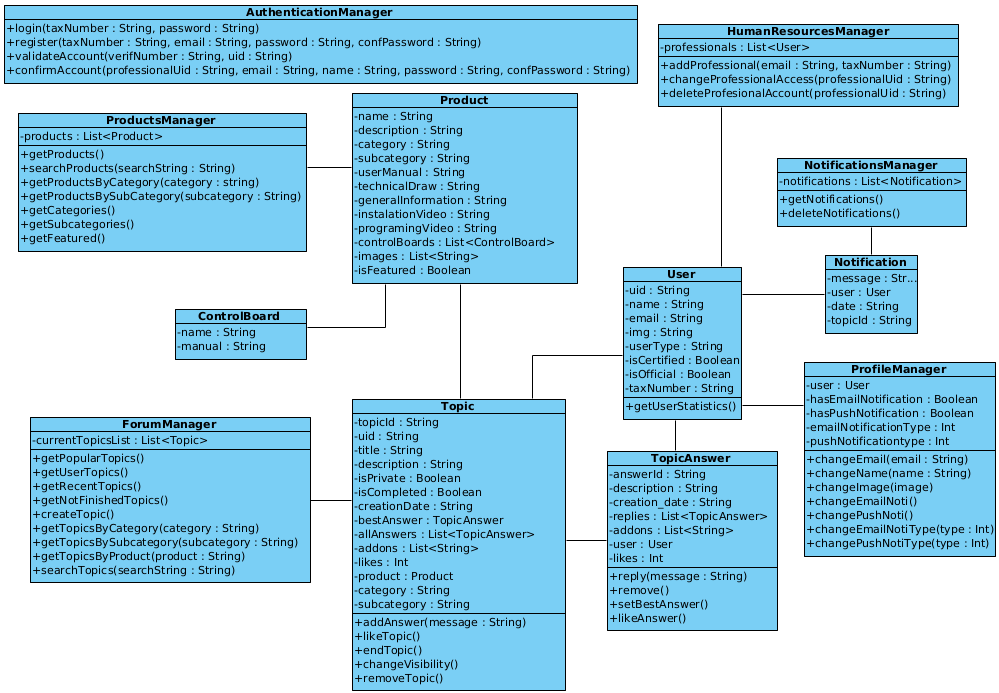
\includegraphics[width=\textwidth]{images/diagramas/diagrama_classes.png}
  \caption{Diagrama de classes Install\&Go}
  \label{fig:22}
\end{figure}


 \newpage

 \section{Mockups}
Com o propósito de criar um \textit{design} para seguir e apresentar às partes interessadas antes de iniciar a fase de desenvolvimento, então foram realizadas \textit{mockups} do \textit{design} da aplicação. Este \textit{design} foi iterativamente revisto pelo cliente e ajustado até alcançar o estado final.

\subsection{Página Inicial}

A página inicial da aplicação, dá ao utilizador a possibilidade de navegar pelos produtos do catálogo, filtrar por categorias e subcategorias, assim como realizar uma pesquisa rápida e por fim navegar para o fórum. Caso um técnico esteja com sessão iniciada este poderá visualizar o \textit{icon} de notificações e a sua imagem de perfil.

\begin{figure}[htb]
    \centering
    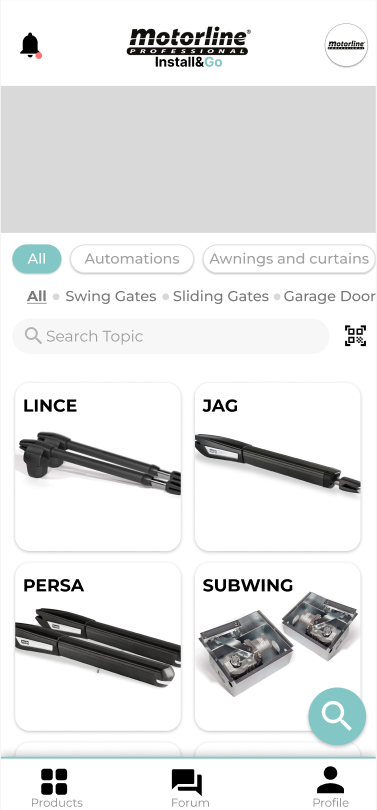
\includegraphics[width=0.45\textwidth]{images/mockups/home_screen.png}
    \caption{Página inicial do fórum}
    \label{fig:23}
\end{figure}

\newpage

\subsection{Autenticação - Login e Registo}

Na autenticação, é possível iniciar sessão e registo, mas a empresa é a única entidade poderá realizar o registo no \textit{software}.

\begin{figure}[htb]%
    \centering
    \subfloat[\centering Página de login]{{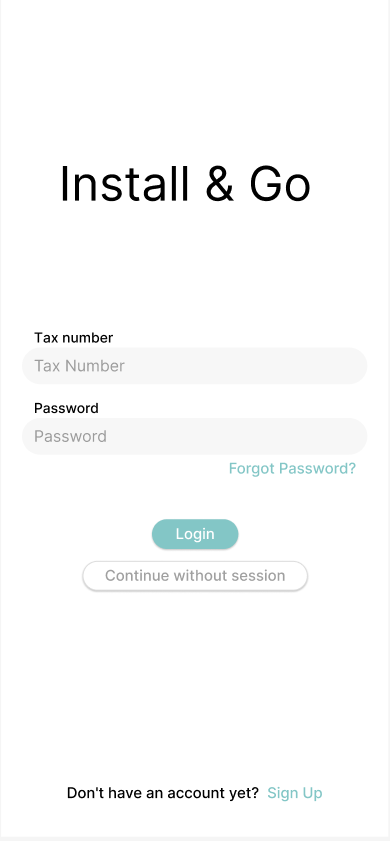
\includegraphics[width=0.4\textwidth]{images/mockups/login.png} }}%
    \qquad
    \subfloat[\centering Página de registo]{{
\includegraphics[width=0.4\textwidth]{images/mockups/register.png} }}%
    \caption{Autenticação - Login e Registo}%
    \label{fig:24}
\end{figure}

\newpage

\subsection{Autenticação - Ativação e Confirmação de conta}

Na autenticação também existe a página de confirmação de conta. Um técnico que tem a conta recentemente adicionada poderá confirmar o registo, indicar as informações finais e por fim será direcionado para a página de ativação onde terá de colocar o código de ativação enviado para o \textit{email}, esta página também será aberta caso um técnico realize o \textit{login} com uma conta que não foi ativada ou sempre que um registo é finalizado.

\begin{figure}[htb]%
    \centering
    \subfloat[\centering Página de confirmação de conta]{{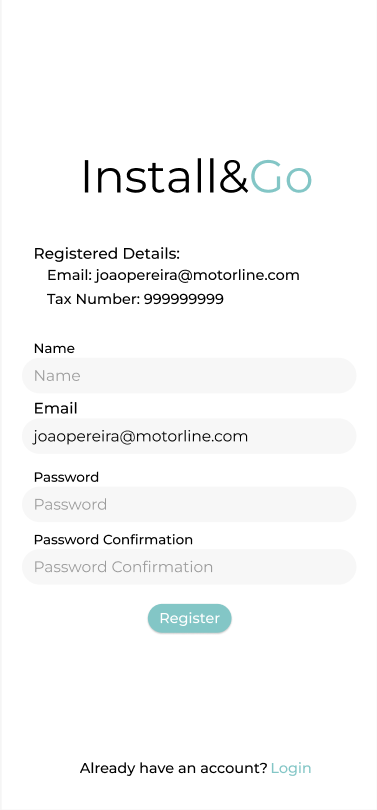
\includegraphics[width=0.4\textwidth]{images/mockups/account_confirmation.png} }}%
    \qquad
    \subfloat[\centering Página de ativação de conta]{{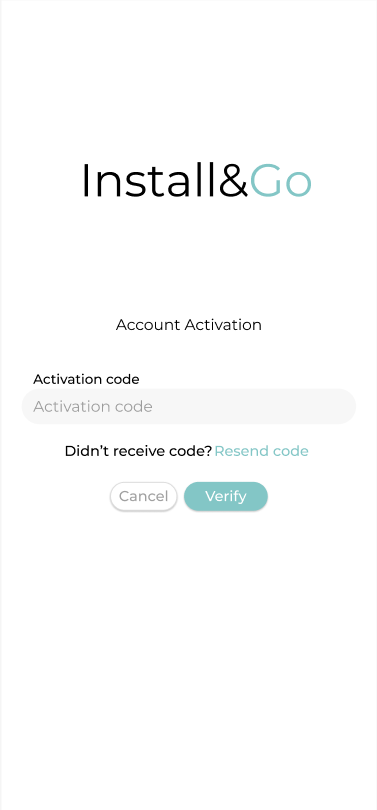
\includegraphics[width=0.4\textwidth]{images/mockups/account_verification.png} }}%
    \caption{Autenticação - Ativação e Confirmação de conta}%
    \label{fig:25}%
\end{figure}

\newpage

\subsection{Página inicial fórum}

O técnico assim que se dirige ao fórum entrará na página inicial. Esta página permite navegar entre as diferentes listagens de tópicos acessíveis ao técnico, pesquisar, filtrar por tipo e criar um novo tópico.

\begin{figure}[htb]
    \centering
    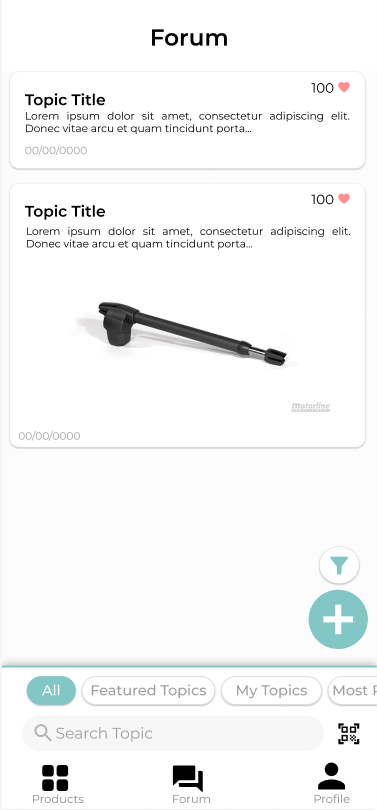
\includegraphics[width=0.45\textwidth]{images/mockups/forum_home.png}
    \caption{Página inicial do fórum}
    \label{fig:26}
\end{figure}

\newpage

\subsection{Página de detalhes de um tópico}

Assim que o técnico seleciona um tópico, será encaminhado para a página de detalhes, onde é indicado o nome do proprietário, a imagem de perfil, a hora de criação, a quantidade de gostos, o título, a descrição, as imagens e os comentários. É possível gostar do tópico, gostar de comentários, comentar o tópico e outros comentários.

Se o tópico for do técnico que está a visualizar, poderá também concluir, eliminar e alterar a sua visibilidade.

\begin{figure}[htb]%
    \centering
    \subfloat[\centering Página de detalhes de um tópico]{{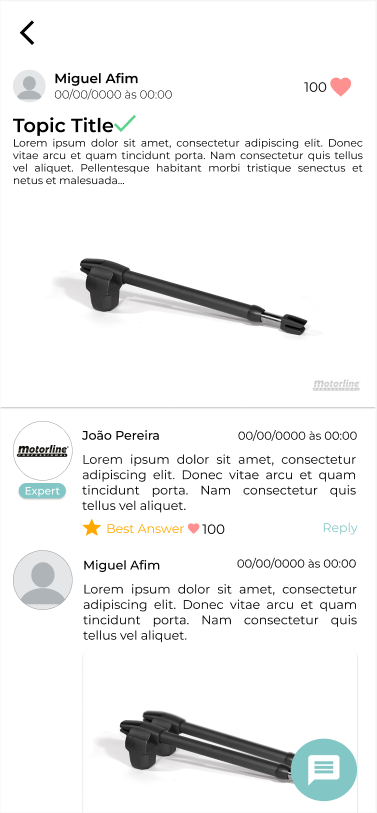
\includegraphics[width=0.4\textwidth]{images/mockups/topic_not_user.png} }}%
    \qquad
    \subfloat[\centering Página de detalhes de um tópico do técnico]{{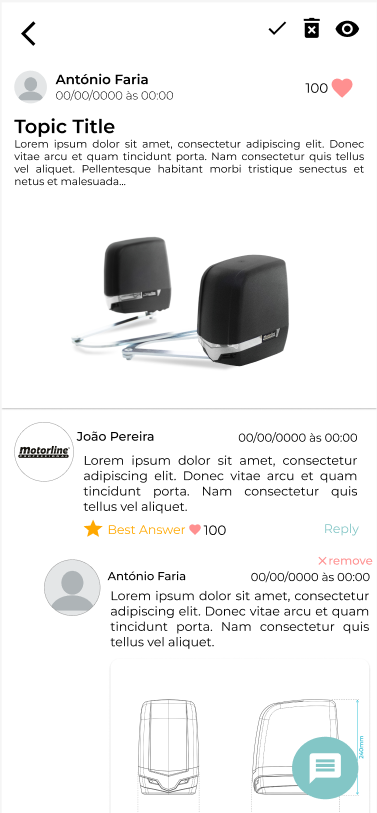
\includegraphics[width=0.4\textwidth]{images/mockups/user_topic.png} }}%
    \caption{Página de detalhes de tópico do software}%
    \label{fig:27}%
\end{figure}

\newpage

\subsection{Página de criação de um tópico}

Quando um técnico inicia a criação de um tópico, é obrigado a inserir o título e a descrição. Já a indicação da visibilidade, do tipo de tópico, do produto referente e de imagens é opcional. A qualquer momento poderá cancelar ou confirmar a ação.

\begin{figure}[htb]
    \centering
    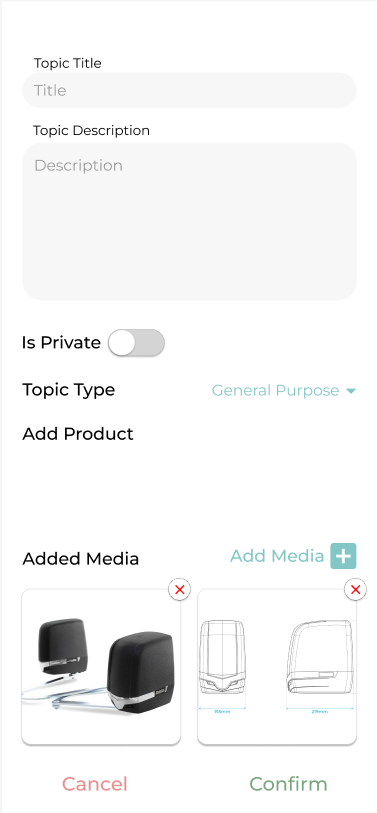
\includegraphics[width=0.45\textwidth]{images/mockups/forum_create_topic.png}
    \caption{Página de criação de tópico}
    \label{fig:28}
\end{figure}

\newpage

\subsection{Página de notificações}

Um técnico sempre que desejar tem como opção visualizar as suas notificações. Neste ecrã, é possível ver todas com a identificação de quem enviou, qual a descrição e a data de receção. O técnico, também tem como escolha apagar se assim desejar.

\begin{figure}[htb]
    \centering
    
\includegraphics[width=0.45\textwidth]{images/mockups/notifications.png}
    \caption{Página de notificações}
    \label{fig:29}
\end{figure}

\newpage

\subsection{Página de perfil de utilizador}

O técnico, sempre que desejar alterar as suas informações, tem a possibilidade de modificar o \textit{email}, a imagem de perfil e a configuração das notificações com indicação dos métodos e tipo a receber.

Caso uma empresa entre no perfil, esta visualizará um botão para aceder à gestão de recursos humanos.

\begin{figure}[htb]
    \centering
    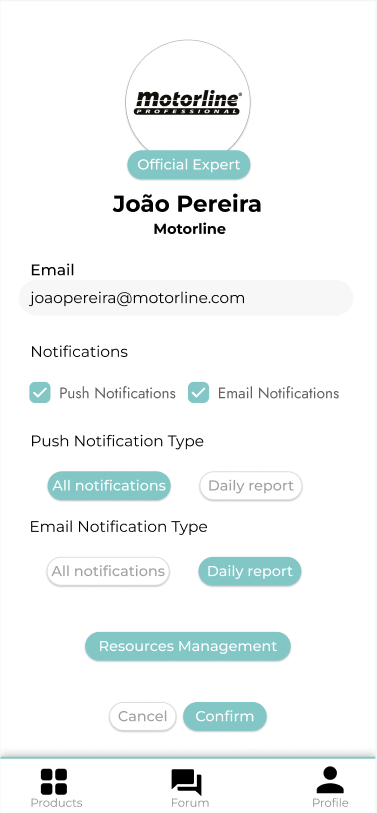
\includegraphics[width=0.45\textwidth]{images/mockups/user_profile.png}
    \caption{Página de perfil de utilizador}
    \label{fig:30}
\end{figure}

\newpage

\subsection{Página de gestão de recursos humanos}

Na página de gestão de recursos humanos, apenas acessível a empresas, é possível registar novos técnicos, pesquisar e gerir os que já se encontram registados através dos seus perfis.

\begin{figure}[htb]
    \centering
    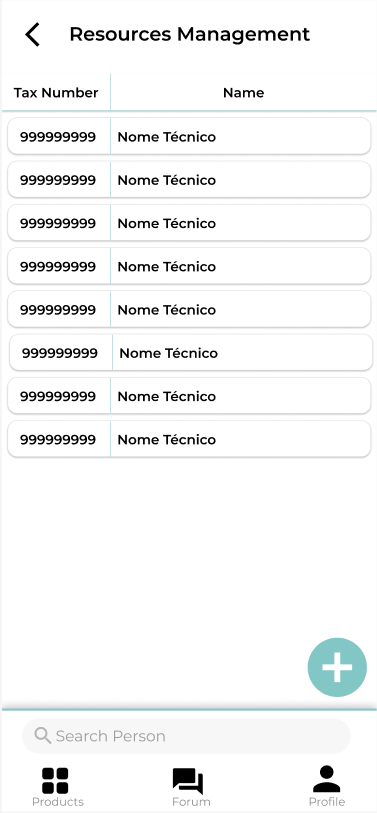
\includegraphics[width=0.45\textwidth]{images/mockups/human_resources.png}
    \caption{Página de gestão de recursos humanos}
    \label{fig:31}
\end{figure}

\newpage

\subsection{Página de perfil de técnico registado}

O perfil de técnico, apenas acessível para empresas, permite visualizar as estatísticas, as informações e permite impedir acesso à conta ou então remover da plataforma.

\begin{figure}[htb]
    \centering
    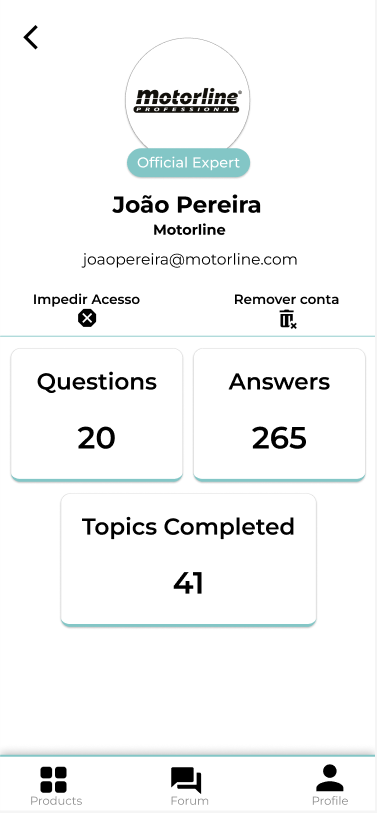
\includegraphics[width=0.45\textwidth]{images/mockups/professional_profile.png}
    \caption{Página de perfil de técnico registado}
    \label{fig:32}
\end{figure}

\newpage

\subsection{Página de registo de novo técnico}

Sempre que uma empresa deseja registar um novo técnico, esta deverá indicar o nome, o \textit{email} e tipo de técnico.

\begin{figure}[htb]
    \centering
    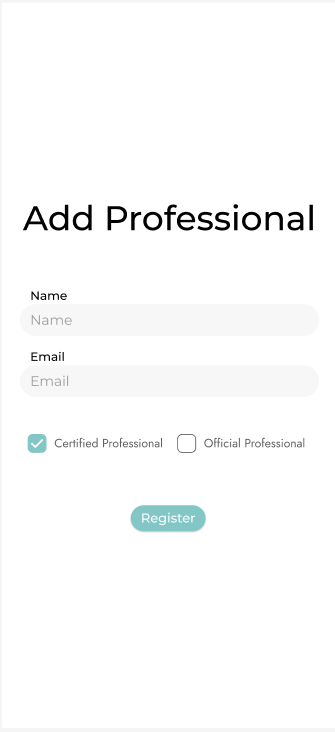
\includegraphics[width=0.45\textwidth]{images/mockups/account_registering.png}
    \caption{Página de registo de novo técnico}
    \label{fig:33}
\end{figure}

 \section{Diagramas de atividades}
O detalhe de forma simples das ações do ator nos diferentes ecrãs foi realizado em diagramas de atividades.

\subsection{Diagrama de atividades página inicial}

Da página inicial da aplicação é possível deslocar para o fórum, para as notificações, para o perfil e realizar operações do catálogo.

\begin{figure}[htb]
  \centering
  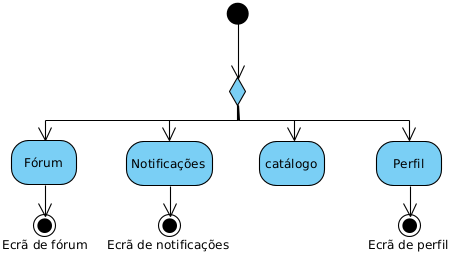
\includegraphics[width=0.6\textwidth]{images/diagramas/atividades/diagrama_atividades_home.png}
  \caption{Diagrama de atividades de página inicial da aplicação}
  \label{fig:34}
\end{figure}

\subsection{Diagrama de atividades página de perfil}

Na página de perfil, é possível alterar a imagem, o nome, o \textit{email}, selecionar os métodos e os tipos de notificação a receber. Caso uma empresa veja o perfil esta poderá, além das operações acima mencionadas, gerir os recursos humanos onde é encaminhada para o ecrã de gestão de recursos humanos.

\begin{figure}[htb]
  \centering
  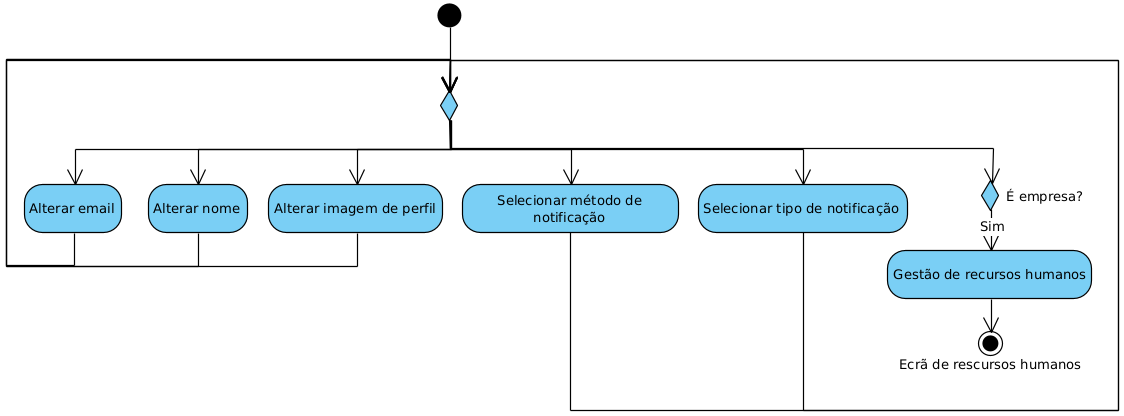
\includegraphics[width=\textwidth]{images/diagramas/atividades/diagrama_atividades_perfil.png}
  \caption{Diagrama de atividades de página de perfil}
  \label{fig:35}
\end{figure}

\newpage

\subsection{Diagrama de atividades página inicial do fórum}

Na página inicial do fórum o técnico poderá selecionar um dos tipos de pesquisa, escrita ou código QR, filtrar por tipo, ver as listagens de tópicos em destaque, mais recentes, por responder, os seus tópicos e criar um novo tópico. Estas listagens poderão ser filtradas por tipo e sobre as mesmas tem a possibilidade de selecionar um tópico o que o redirecionará para o ecrã de detalhes.

\begin{figure}[htb]
  \centering
  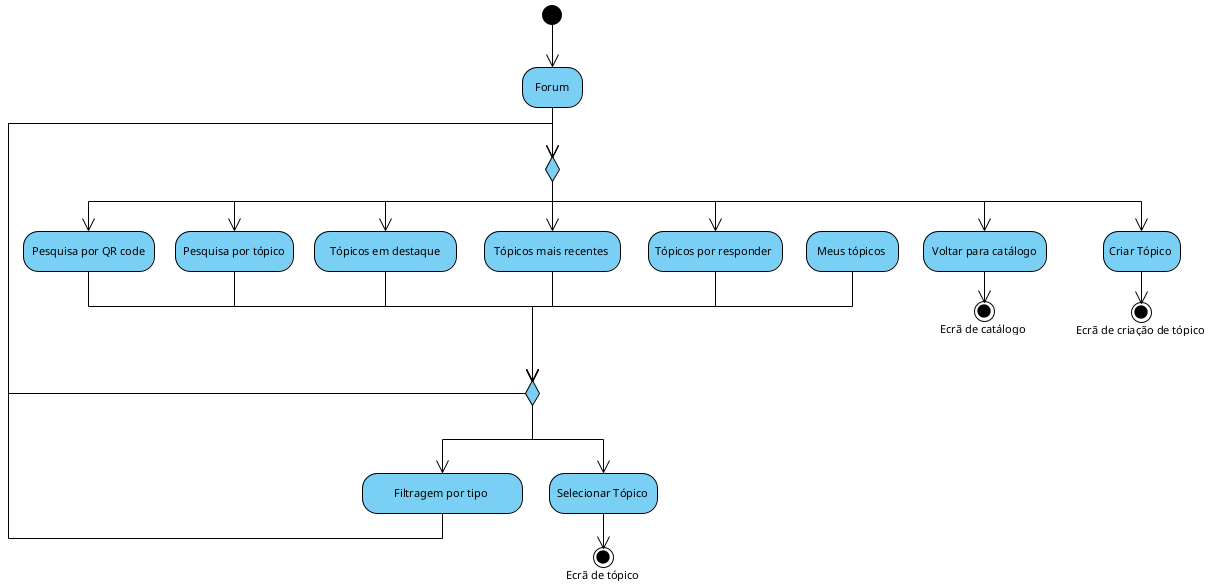
\includegraphics[width=\textwidth]{images/diagramas/atividades/diagrama_atividades_forum.png}
  \caption{Diagrama de atividades de página inicial do fórum}
  \label{fig:36}
\end{figure}

\newpage

\subsection{Diagrama de atividades página de criação de tópico}

Quando o técnico decide criar um tópico, obrigatoriamente tem de indicar o título, a descrição e o tipo do tópico. Por predefinição a visibilidade deste é pública, mas o técnico poderá alterar. Facultativamente o técnico poderá indicar o produto referente ao tópico, assim como anexar e remover imagens. A qualquer momento, o técnico poderá confirmar a criação do tópico, quando esta ação inicia, é realizada uma verificação do título e da descrição para concluir se estão preenchidos. Caso estes dados não estejam preenchidos é indicado ao técnico que as informações estão em falta, caso contrário este volta para o ecrã anterior.

\begin{figure}[htb]
  \centering
  \includegraphics[width=0.7\textwidth]{images/diagramas/atividades/diagrama_atividades_criar_tópico.png}
  \caption{Diagrama de atividades de página de criação de tópico}
  \label{fig:37}
\end{figure}

\newpage

\subsection{Diagrama de atividades página de detalhes do tópico}

Assim que o técnico seleciona um tópico, este poderá visualizar todos os comentários, apagar um caso seja seu, gostar do tópico e/ou de uma resposta, comentar e responder a um comentário. Caso o tópico seja do técnico, este poderá também alterar a visibilidade, marcar como concluído ou remover. A qualquer momento, o técnico tem como possibilidade retroceder para o ecrã anterior.

\begin{figure}[htb]
  \centering
  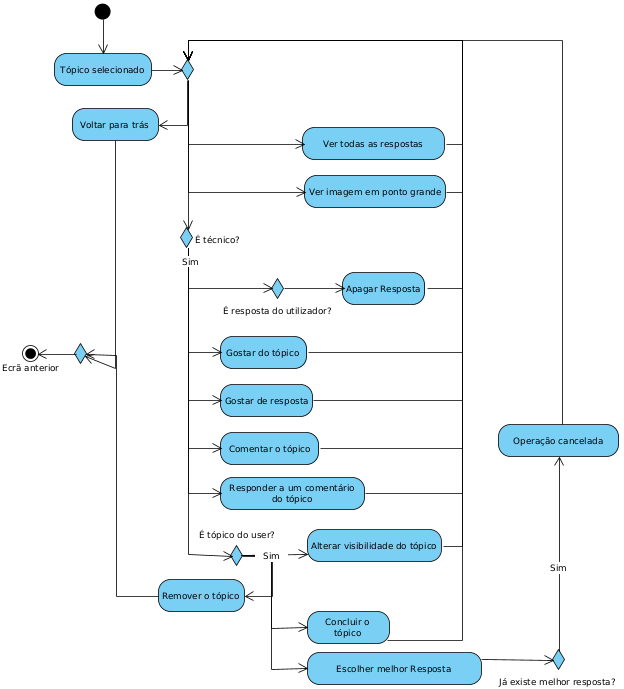
\includegraphics[width=0.9\textwidth]{images/diagramas/atividades/diagrama_atividades_detalhes_topico.png}
  \caption{Diagrama de atividades de página de detalhes do tópico}
  \label{fig:38}
\end{figure}

\newpage

\subsection{Diagrama de atividades páginas de autenticação}

Para realizar a ativação da conta do técnico, assim que este realiza o registo, confirmação da conta ou o login com uma conta que não se encontra ativa, este é encaminhado para o ecrã de ativação da conta. Neste ecrã poderá cancelar e indicar o código de ativação. Se o código estiver errado, o técnico deverá inserir-lo novamente. Por outro lado, se inserir um código correto a conta será validada e o técnico ficará autenticado. Também, em caso de necessidade, o proprietário da conta terá como opção pedir o envio de um novo código de ativação.

\begin{figure}[htb]
  \centering
  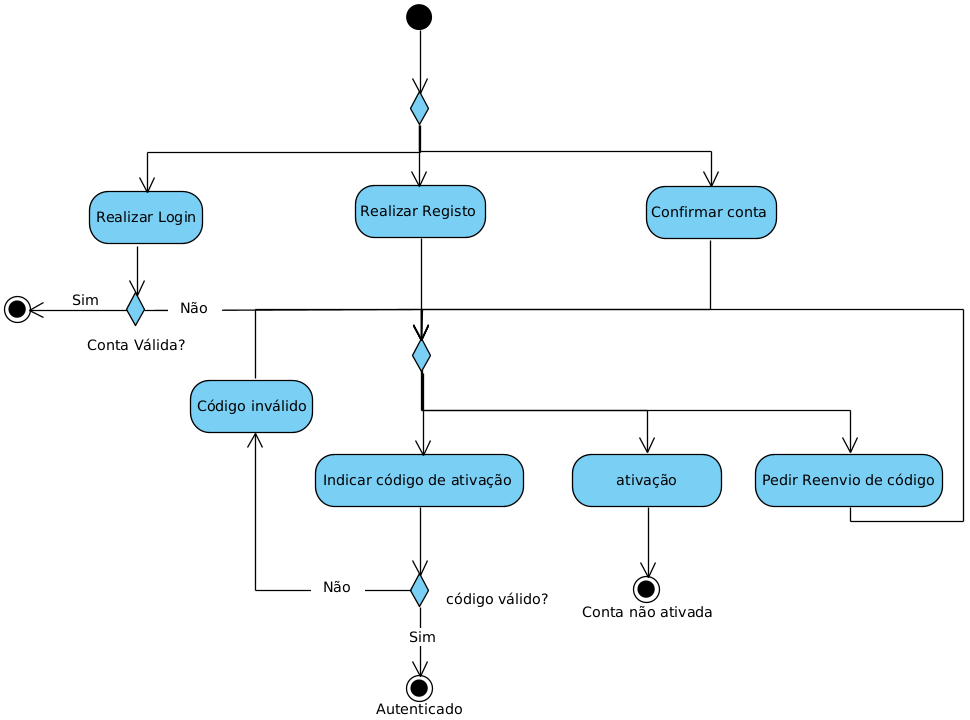
\includegraphics[width=0.8\textwidth]{images/diagramas/atividades/diagrama_atividades_autenticação.png}
  \caption{Diagrama de atividades de página de validação de conta}
  \label{fig:39}
\end{figure}

\newpage

% \subsection{Diagrama de atividades página de notificações}

% Sempre que o técnico recebe uma notificação, este poderá ver esta notificação no ecrã de notificações, 
% Este ecrã permite ao utilizador selecionar uma notificação sendo redirecionado para o tópico referente,
% caso esta esteja referente a um tópico, ou então poderá apagar a notificação.

% \begin{figure}[htb]
%   \centering
%   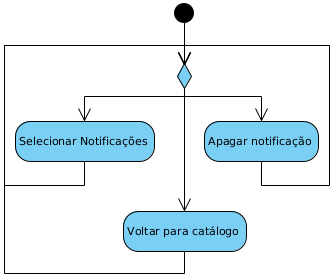
\includegraphics[width=0.5\textwidth]{images/diagramas/atividades/diagrama_atividades_noti.png}
%   \caption{Diagrama de atividades de página de notificações}
%   \label{fig:27}
% \end{figure}

% \subsection{Diagrama de atividades gestão de recursos humanos}

% Uma empresa poderá gerir as contas dos seus recursos humanos, para isso deverá se dirigir a este ecrã.
% Neste ecrã é possível registar um novo técnico sendo encaminhada para o ecrã de registo de técnico, 
% selecionar um técnico sendo encaminhada para o ecrã de perfil do técnico e poderá também pesquisar por 
% técnico.

% \begin{figure}[htb]
%   \centering
%   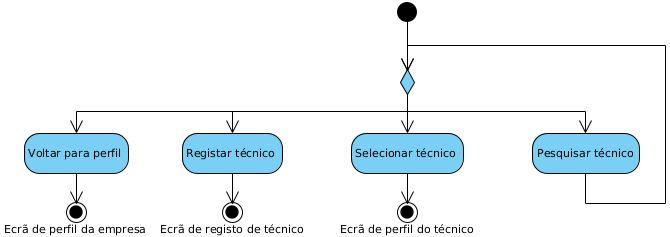
\includegraphics[width=\textwidth]{images/diagramas/atividades/diagrama_atividades_human_resources.png}
%   \caption{Diagrama de atividades de página de recursos humanos}
%   \label{fig:29}
% \end{figure}


% \subsection{Diagrama de atividades perfil de técnico}

% Sempre que uma empresa seleciona um técnico, esta é encaminhada para o ecrã de perfil de técnico. Neste 
% ecrã é possível impedir acesso à plataforma e remover a conta de técnico da plataforma.

% \begin{figure}[htb]
%   \centering
%   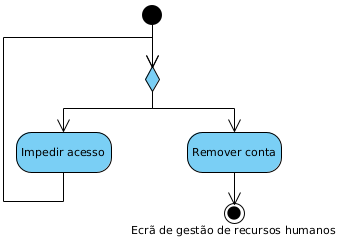
\includegraphics[width=0.5\textwidth]{images/diagramas/atividades/diagrama_atividades_prof_profile.png}
%   \caption{Diagrama de atividades de página de perfil de técnico}
%   \label{fig:30}
% \end{figure}

\newpage

\subsection{Diagrama de atividades registar técnico}

Assim que uma empresa inicia o registo de um técnico, esta é redirecionada para a página de registo do técnico. Nesta página, terá de indicar o nome, o \textit{email} e o tipo de técnico. Por fim será capaz de confirmar o registo da conta e automaticamente a empresa é movida para a página anterior.

\begin{figure}[htb]
  \centering
  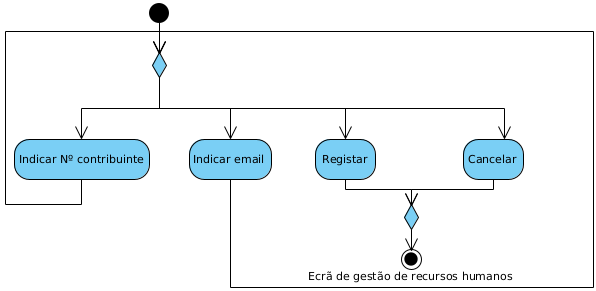
\includegraphics[width=0.8\textwidth]{images/diagramas/atividades/diagrama_atividades_add_professional.png}
  \caption{Diagrama de atividades de página de registar técnico}
  \label{fig:31}
\end{figure}

\subsection{Diagrama de atividades confirmar conta}

Quando uma conta de técnico é registada, um \textit{email} de confirmação é enviado para o técnico. Assim que este o recebe, deverá clicar em confirmar a conta. A partir desta ação, este move-se para a página de confirmação da conta. Nesta página, o técnico poderá alterar o seu \textit{email}, indicar o nome, a \textit{password} e a confirmação da \textit{password}.Todo o processo termina quando o botão de registar for pressionado.

\begin{figure}[htb]
  \centering
  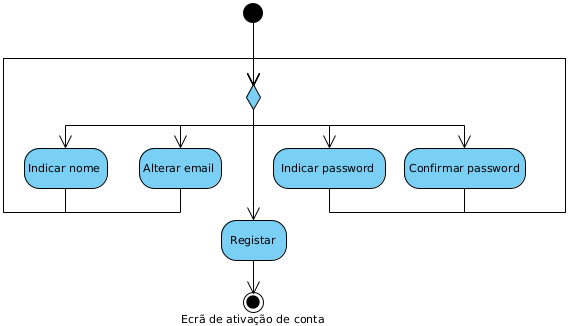
\includegraphics[width=0.8\textwidth]{images/diagramas/atividades/diagrama_atividades_prof_register.png}
  \caption{Diagrama de atividades de página de confirmar conta de técnico}
  \label{fig:31}
\end{figure}

 \section{Diagramas de estados}
Para especificar os principais processos do projeto foram então desenvolvidos diagramas de estados,
sendo então pretendido demonstrar o processo de criação de um tópico do fórum por parte de um técnico, o 
processo de aceder e responder a um tópico e o login com ativação de conta
visto que estas interações são as de maior significância e regradas no software.

\subsection{Diagrama de estados criação de tópico}

Com o diagrama de estados de criação de tópico é pretendido demonstrar o processo de criação de um tópico 
por parte de um técnico. Assim sendo este primeiramente terá de estar autenticado, caso não esteja 
este será encaminhado para autenticação. De seguida criará tópico, após preencher os 
campos desejados este poderá confirmar o tópico, caso confirme é verificado se o tópico possui título, 
caso não possua, é invalido pelo que o técnico deverá preencher os dados em falta, caso o 
título esteja preenchido é verificado se possui descrição e tipo, caso não possua é seguido o mesmo fluxo que o 
caso anterior, caso contrário é criado um tópico. Se o técnico não desejar confirmar o tópico ele 
poderá cancelar, quando assim o faz este torna-se cancelado.

\begin{figure}[htb]
    \centering
    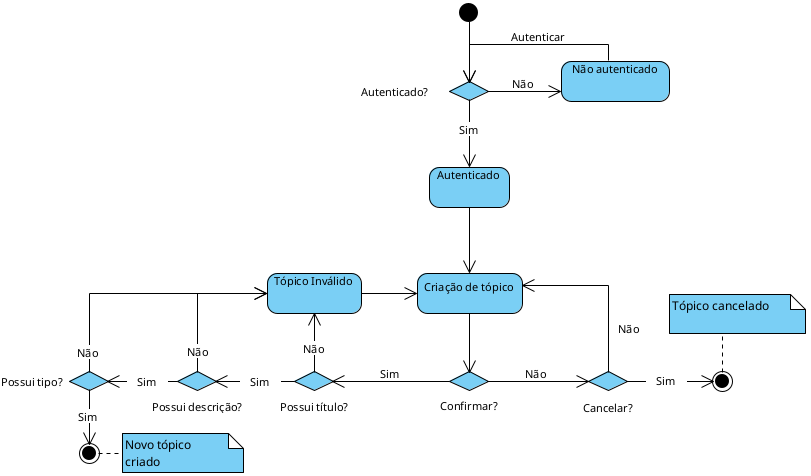
\includegraphics[width=0.9\textwidth]{images/diagramas/estados/criar_topico.png}
    \caption{Diagrama de estados de criar tópico}
    \label{fig:27}
\end{figure}

\newpage

\subsection{Diagrama de estados responder a tópico}

Com o diagrama de estados de responder a tópico é pretendido demonstrar o processo de seleção e 
responder a um tópico por parte de um técnico. Assim sendo que o técnico primeiramente deverá estar 
autenticado, caso não esteja este será encaminhado para a autenticação. Após a autenticação o técnico 
estará autenticado e irá por predefinição ver tópicos em destaque, nesta listagem este selecionará um 
tópico ficando assim o tópico 
selecionado. Assim que o tópico se encontra selecionado o técnico conseguirá responder a este criando 
um comentário. Após a criação do comentário este poderá confirmar o comentário, caso confirme o 
comentário ficará criado, caso contrário este comentário ficará cancelado.

\begin{figure}[htb]
    \centering
    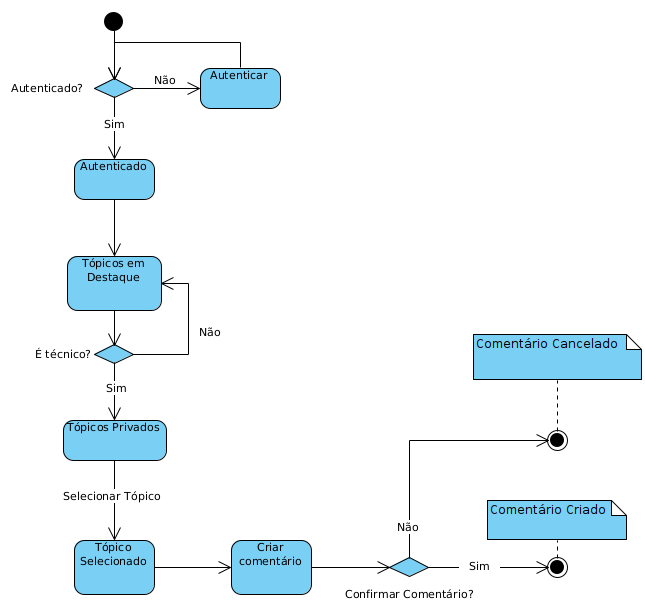
\includegraphics[width=0.7\textwidth]{images/diagramas/estados/responder_topico_tecnico.png}
    \caption{Diagrama de estados de criar tópico}
    \label{fig:28}
\end{figure}

\newpage

\subsection{Diagrama de estados autenticação e validação de conta}

Assim que o técnico decide realizar o login na aplicação este indica as suas credenciais, caso estas 
credenciais não estejam corretas, a autenticação será incorreta e deverá alterar as credenciais. 
Caso as credenciais estejam corretas e a conta válida o técnico ficará autenticado, caso contrário o 
este terá uma conta inválida, pelo que deverá ser validada, para  isso o este deverá 
inserir o código de validação, se o código estiver correto, a conta será validada e o técnico 
ficará autenticado, caso contrário o código será invalido e o deverá indicar o seu código de 
validação novamente.

\begin{figure}[htb]
    \centering
    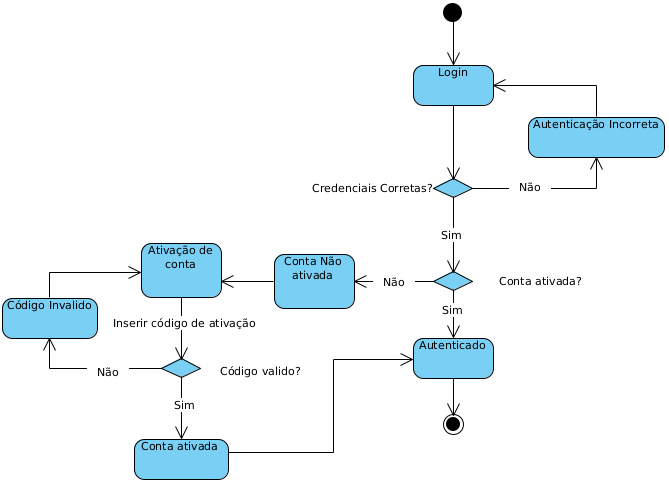
\includegraphics[width=0.7\textwidth]{images/diagramas/estados/autenticacao.png}
    \caption{Diagrama de estados de autenticação e validação de conta}
    \label{fig:29}
\end{figure}


 \newpage

 \newpage

\section{Diagrama de sequência}

Visto que a realização da autenticação, ativação e confirmação de conta requer passos extras e regras a seguir, 
foi necessário criar diagramas de sequência para especificar a sequência de interações do com o sistema.

\subsection{Diagrama de sequência Login e ativação de conta}

Através deste diagrama (Figura~\ref{fig:43}) é entende-se que assim que o técnico deseja realizar o 
login, primeiramente tem de verificar as credenciais, caso estas se encontrem incorretas, este receberá 
uma mensagem de erro, caso as credenciais estejam válidas e a conta esteja ativada o técnico ficará 
autenticado. 

Caso o técnico coloque as credenciais corretas, mas a conta não esteja ativada, este irá realizar a 
ativação de conta, onde poderá enviar o código de ativação, caso esteja correto a sua conta será 
ativada, caso contrário este receberá uma mensagem de erro. Este poderá também cancelar a 
ativação de conta e pedir um novo \textit{email} de ativação, onde será pedido novo código ao servidor, 
este será gerado e enviado.

\begin{figure}[htb]
    \centering
    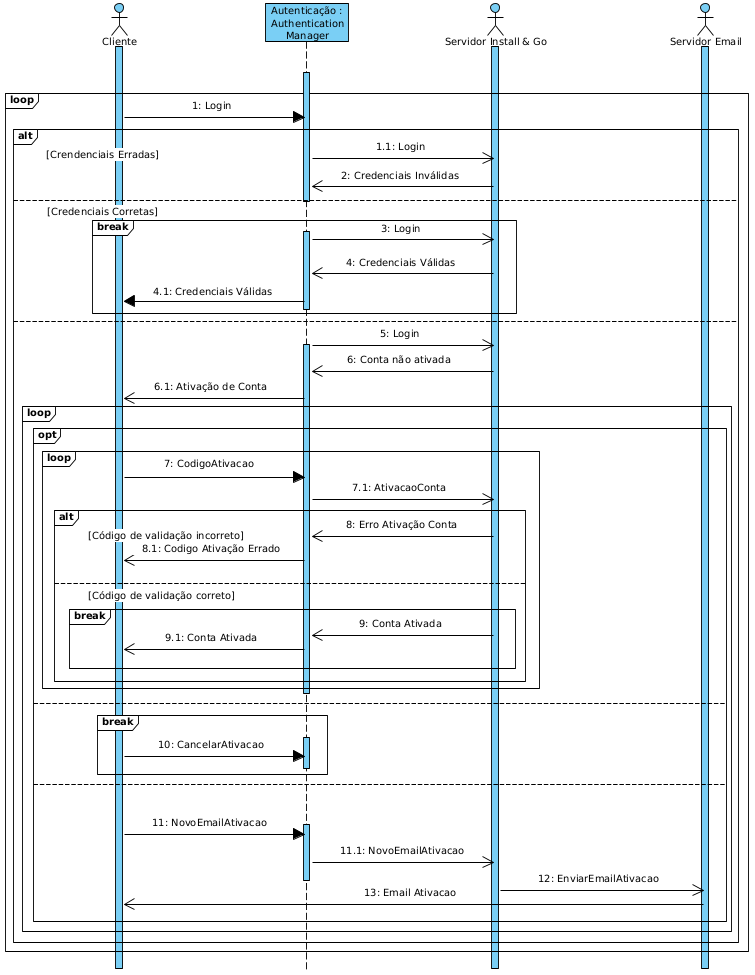
\includegraphics[width=0.67\textwidth]{images/diagramas/sequencia/diagrama_login.png}
    \caption{Diagrama de sequência de login e ativação de conta}
    \label{fig:43}
\end{figure}

\newpage

\subsection{Diagrama de sequência Registo e ativação de conta}

Através do diagrama abaixo representado (Figura~\ref{fig:44}) é possível perceber que quando uma
empresa realiza o registo este será enviado para o servidor, o qual registará a empresa com uma 
conta não ativada, esta conta será então validada pela Motorline sendo de seguida
gerado um código de ativação e enviado por \textit{email} para o 
\textit{email} de registo, após isto a empresa será encaminhado para a validação de conta, esta validação 
ocorre seguindo o mesmo processo mencionado no anteriormente.


\begin{figure}[htb]
    \centering
    \includegraphics[width=0.8\textwidth]{images/diagramas/sequencia/diagrama_registo.png}
    \caption{Diagrama de sequência de registo e validação de conta}
    \label{fig:44}
\end{figure}

\newpage

\subsection{Diagrama de sequência registo de técnicos}

Através do diagrama abaixo representado (Figura~\ref{fig:45}) é possível perceber que quando uma
empresa deseja registar um técnico, esta introduzirá os seus dados, sendo a sua conta criada. Após isto, 
um código de ativação é gerado e enviado para o técnico ativar a sua conta.

\begin{figure}[htb]
    \centering
    \includegraphics[width=0.8\textwidth]{images/diagramas/sequencia/registo_tecnico.png}
    \caption{Diagrama de sequência de registo de técnicos}
    \label{fig:45}
\end{figure}